\documentclass[12pt, a4paper]{report}

% --- Official Margins (PST Guidelines: Left 4.0cm, Top/Bottom/Right 2.5cm) ---
\usepackage[left=4.0cm, right=2.5cm, top=2.5cm, bottom=2.5cm]{geometry}

% --- Font & Line Spacing ---
\usepackage{times}          % Times New Roman
\usepackage{setspace}
\onehalfspacing             % 1.5 line spacing

% --- Paragraph Spacing & No Indentation ---
\usepackage{parskip}

% --- Mathematical & Graphic Packages ---
\usepackage{amsmath, amssymb, amsfonts}
\usepackage{graphicx}
\usepackage{booktabs}
\usepackage{float}
\usepackage{caption}
\usepackage{hyperref}
\usepackage{microtype}
\usepackage{array}
\usepackage{tikz}
\usetikzlibrary{shapes.multipart, shapes.geometric, arrows.meta, positioning, calc}
\usepackage{listings}
\usepackage{color}
\usepackage{tabularx}
\usepackage{titlesec}
\usepackage[titles]{tocloft}
\renewcommand{\cftdotsep}{0.5} % Tighten dots (virtually no gap) in TOC/LOF/LOT

% Define custom column types for tabularx
\newcolumntype{L}{>{\raggedright\arraybackslash}X}
\newcolumntype{C}{>{\centering\arraybackslash}X}

% Capitalize Generated Preliminary Headings
\renewcommand{\contentsname}{CONTENTS}
\renewcommand{\listfigurename}{LIST OF FIGURES}
\renewcommand{\listtablename}{LIST OF TABLES}

% Format chapter titles to be 16pt and centered
\titleformat{\chapter}[display]
  {\normalfont\fontsize{16}{20}\selectfont\bfseries\centering}
  {\MakeUppercase{\chaptertitlename}\ \thechapter}
  {0.5ex}
  {\fontsize{16}{20}\selectfont\centering}
\titlespacing*{\chapter}{0pt}{-20pt}{20pt}

% Format numberless chapters (preliminary pages, references, appendices) to be 16pt and left-aligned
\titleformat{name=\chapter,numberless}[block]
  {\normalfont\fontsize{16}{20}\selectfont\bfseries}
  {}
  {0pt}
  {\fontsize{16}{20}\selectfont}
\titlespacing*{name=\chapter,numberless}{0pt}{-20pt}{20pt}

% Format section titles (consistent size)
\titleformat{\section}
  {\normalfont\large\bfseries}
  {\thesection}
  {1em}
  {}
\titlespacing*{\section}{0pt}{3.5ex plus 1ex minus .2ex}{2.3ex plus .2ex}

% Format subsection titles (smaller size)
\titleformat{\subsection}
  {\normalfont\normalsize\bfseries}
  {\thesubsection}
  {1em}
  {}
\titlespacing*{\subsection}{0pt}{3.25ex plus 1ex minus .2ex}{1.5ex plus .2ex}

\definecolor{codegreen}{rgb}{0,0.6,0}
\definecolor{codegray}{rgb}{0.5,0.5,0.5}
\definecolor{codepurple}{rgb}{0.58,0,0.82}
\definecolor{backcolour}{rgb}{0.95,0.95,0.92}

\lstdefinestyle{mystyle}{
    backgroundcolor=\color{backcolour},   
    commentstyle=\color{codegreen},
    keywordstyle=\color{magenta},
    numberstyle=\tiny\ttfamily\color{codegray},
    stringstyle=\color{codepurple},
    basicstyle=\ttfamily\small,
    breakatwhitespace=false,         
    breaklines=true,                 
    captionpos=b,                    
    keepspaces=true,                 
    numbers=left,                    
    numbersep=5pt,                  
    showspaces=false,                
    showstringspaces=false,
    showtabs=false,                  
    tabsize=2
}
\lstset{style=mystyle}


% --- Header & Footer (Page Numbering Bottom Right) ---
\usepackage{fancyhdr}
\pagestyle{fancy}
\fancyhf{}
\rfoot{\thepage}
\renewcommand{\headrulewidth}{0pt}
\fancypagestyle{plain}{
    \fancyhf{}
    \rfoot{\thepage}
    \renewcommand{\headrulewidth}{0pt}
}

% --- Hyperlink Settings ---
\hypersetup{
    colorlinks=true,
    linkcolor=black,
    citecolor=black,
    urlcolor=blue
}

% --- Rename Bibliography to REFERENCES ---
\renewcommand{\bibname}{REFERENCES}

\begin{document}

% ==========================================
% PRELIMINARY PAGES (Roman Numerals: i, ii, iii...)
% ==========================================
\pagenumbering{roman}

% Page i: Title Page
\begin{titlepage}
    \centering
    \vspace*{1.5cm}
    
    {\Large\bfseries A WORKLOAD-AWARE DYNAMIC ARRAY GROWTH ALGORITHM FOR EFFICIENT MEMORY ALLOCATION \par}
    
    \vspace{2.5cm}
    
    {\large\bfseries P.M.D.C.H. Perera \par}
    
    \vspace{0.2cm}

    {\large\bfseries 20APP5029 \par}
    
    \vspace{2.5cm}
    
    {\large A dissertation submitted in partial fulfilment of the requirements for the \par}
    {\large Bachelor of Science Honours Degree Examination \par}
    {\large In \par}
    {\large\bfseries Computer Science and Technology \par}
    
    \vfill
    
    {\large Department of Physical Sciences and Technology, \par}
    {\large Faculty of Applied Sciences, \par}
    {\large Sabaragamuwa University of Sri Lanka \par}
    {\large Sri Lanka. \par}
    
    \vspace{1cm}
    
    {\large 2020/2021 \par}
\end{titlepage}


% Page ii: Declaration
\chapter*{DECLARATION}
\addcontentsline{toc}{chapter}{DECLARATION}

I declare that this Report does not incorporate, without acknowledgment, any material previously submitted for a degree or a Diploma in any University and to the best of my knowledge and belief, it does not contain any material previously published or written by another person or myself except where due reference is made in the text.

Also, I hereby grant to Sabaragamuwa University of Sri Lanka the non-exclusive right to reproduce and distribute my Report, in whole or in part in print, electronic or other medium. I retain the right to use this content in whole or part in future works (such as articles or books).

\vspace{4cm}

\noindent
\begin{minipage}{0.45\textwidth}
    \dotfill \\
    Date
\end{minipage}
\hfill
\begin{minipage}{0.45\textwidth}
    \dotfill \\
    Signature
\end{minipage}


% Page iii: Certification of Approval
\chapter*{CERTIFICATION OF APPROVAL}
\addcontentsline{toc}{chapter}{CERTIFICATION OF APPROVAL}

We hereby declare that this Report is from the student’s own work and effort, and all other sources of information used have been acknowledged. This Report has been submitted with our approval.

\vspace{3cm}

\noindent
\begin{tabularx}{\linewidth}{@{}p{5.5cm}X@{}}
Date: \dotfill & \dotfill \\
& $<\text{Supervisor Name}>$ \\
& Department of Physical Sciences and Technology, \\
& Faculty of Applied Sciences, \\
& Sabaragamuwa University of Sri Lanka.
\end{tabularx}

\vspace{3cm}

\noindent
\begin{tabularx}{\linewidth}{@{}p{5.5cm}X@{}}
Date: \dotfill & \dotfill \\
& Dr. H.N.M. Sarangika \\
& Head of Department, \\
& Department of Physical Sciences and Technology, \\
& Faculty of Applied Sciences, \\
& Sabaragamuwa University of Sri Lanka.
\end{tabularx}


% Page iv: Acknowledgement
\chapter*{ACKNOWLEDGEMENT}
\addcontentsline{toc}{chapter}{ACKNOWLEDGEMENT}

The successful completion of this research would not have been possible without the support, guidance, and encouragement of many individuals and institutions.

First and foremost, I would like to express my deepest gratitude to my supervisor, Ms. A.M.C.M. Aruppola, and my co-supervisor, Dr. C.H. Baduraliya, for their invaluable guidance, continuous encouragement, and insightful feedback throughout this research. Their expertise and direction played a crucial role in shaping the overall outcome of this study.

I am also deeply thankful to Dr. H.N.M. Sarangika, Head of the Department of Physical Sciences and Technology, and Prof. R.M.K.T. Rathnayaka, Dean of the Faculty of Applied Sciences, Sabaragamuwa University of Sri Lanka, for providing the academic environment and resources necessary to carry out this research successfully.

My sincere thanks go to all academic and non-academic staff members of the Department of Physical Sciences and Technology for their constant support during my undergraduate studies.

Finally, I express my heartfelt gratitude to my family and friends for their unwavering support, understanding, and patience throughout this journey.

\vspace{1.5cm}

\noindent P.M.D.C.H. Perera


% Page v: Abstract
\chapter*{ABSTRACT}
\addcontentsline{toc}{chapter}{ABSTRACT}

\begin{center}
{\bfseries A WORKLOAD-AWARE DYNAMIC ARRAY GROWTH ALGORITHM FOR EFFICIENT MEMORY ALLOCATION \par}
\vspace{0.3cm}
{\small P.M.D.C.H. Perera$^{1,*}$, A.M.C.M. Aruppola$^{1}$, C.H. Baduraliya$^{1}$ \par}
\vspace{0.2cm}
{\small\itshape $^{1}$Department of Physical Sciences and Technology, Faculty of Applied Sciences, Sabaragamuwa University of Sri Lanka, P.O. Box 02, Belihuloya, 70140, Sri Lanka \par}
{\small $^{*}$chirathhasara2001@gmail.com \par}
\end{center}

\vspace{0.5cm}

Dynamic arrays are fundamental data structures widely used in modern software for fast random access and dynamic memory allocation. Conventional implementations resize arrays using fixed growth factors (e.g., $1.5\times$ or $2.0\times$), compromising between memory utilization and resizing overhead. Though recent studies explore alternative array organizations to improve memory efficiency, the utilized resizing strategies remain workload-independent, with limited flexibility in adaptation to changes in insertion patterns. This study proposes an adaptive growth strategy combining resize history with runtime workload intensity. The proposed algorithm models the growth factor using a workload-aware harmonic function, $g(k,v) = \min(g_{\max}, \max(g_{\min}, 1 + \frac{c_0 + \lambda \ln(1+v)}{k}))$, where $k$ is the resize count and $v = \frac{\Delta N}{\Delta t}$ is insertion velocity ($\Delta N$ inserted elements per unit time $\Delta t$ between resizes). The resized capacity is $C_{\text{new}} = \lfloor C_{\text{old}} \times g(k,v) \rfloor$. Implemented in Python 3.11 (64-bit integers, initial capacity $C_0 = 10$, $c_0 = 2.0$, $\lambda = 1.0$, $g_{\min} = 1.1$, $g_{\max} = 2.0$), benchmarks were run on an Intel i5 Windows 10 workstation across 10 repeated trials. Evaluation spanned $10^4$--$10^7$ insertions across seven workload patterns (including uniform, burst, and mixed), comparing against fixed ($1.5\times$, $2.0\times$) and Python list ($1.125\times$) policies. This study aimed to identify an optimal configuration that minimized memory waste while maintaining high throughput and limiting element-copying overhead. Under a $10^7$ element mixed workload (10 trials), the proposed strategy achieved 1.28\% memory waste, 32 resizes, 38.76M copied elements, and 6.40M ops/s throughput. Comparatively, Fixed $2.0\times$ yielded 4.63\% waste (20 resizes, 10.49M copies), Fixed $1.5\times$ yielded 27.77\% waste (35 resizes, 27.69M copies), and Python list yielded 4.59\% waste (102 resizes, 83.84M copies). The proposed method significantly reduced memory waste compared to fixed and feedback-unaware baselines ($p < 0.01$) without sacrificing throughput. By combining resize history and workload awareness, the algorithm expands aggressively during burst insertions and adopts conservative growth during lighter workloads. Unlike static resizing policies, this work contributes a workload-sensitive adaptive resizing mechanism for memory-sensitive systems.

\vspace{0.8cm}

\noindent{\bfseries Keywords:} Dynamic arrays, Adaptive resizing, Harmonic growth, Workload-aware memory allocation, Dynamic memory management


% Page vi: Table of Contents
\addcontentsline{toc}{chapter}{CONTENTS}
\tableofcontents

% Page viii: List of Figures
\addcontentsline{toc}{chapter}{LIST OF FIGURES}
\listoffigures

% Page ix: List of Tables
\addcontentsline{toc}{chapter}{LIST OF TABLES}
\listoftables

% Page x: List of Abbreviations and Symbols
\chapter*{LIST OF ABBREVIATIONS AND SYMBOLS}
\addcontentsline{toc}{chapter}{LIST OF ABBREVIATIONS AND SYMBOLS}

\begin{table}[H]
\centering
\begin{tabularx}{\linewidth}{lX}
\textbf{Abbreviation / Symbol} & \textbf{Description} \\
\midrule
\textbf{API} & Application Programming Interface \\
\textbf{BO} & Bayesian Optimization \\
\textbf{CPU} & Central Processing Unit \\
\textbf{CPython} & Reference C Implementation of Python \\
\textbf{CST} & Computer Science and Technology \\
\textbf{GP} & Gaussian Process \\
\textbf{HCI} & Human-Computer Interaction \\
\textbf{IoT} & Internet of Things \\
\textbf{LOF} & List of Figures \\
\textbf{LOT} & List of Tables \\
\textbf{OS} & Operating System \\
\textbf{PST} & Physical Sciences and Technology \\
\textbf{RAM} & Random Access Memory \\
\textbf{STL} & Standard Template Library (C++) \\
\textbf{TOC} & Table of Contents \\
\midrule
$C_0$ & Initial Array Capacity \\
$C_{\text{old}}$ & Current Array Capacity Before Resizing \\
$C_{\text{new}}$ & Allocated Array Capacity After Resizing \\
$k$ & Resize Counter / Iteration History ($k = 1, 2, 3...$) \\
$v$ & Instantaneous Insertion Velocity ($v = \frac{\Delta N}{\Delta t}$) \\
$g(k,v)$ & Dynamic Growth Factor Function \\
$g_{\min}$ & Minimum Allowed Growth Factor Bound ($1.1$) \\
$g_{\max}$ & Maximum Allowed Growth Factor Bound ($2.0$) \\
$\alpha, \alpha_0$ & Logarithmic / Capacity Growth Multiplier \\
$\beta$ & Logarithmic Shift / Dampening Parameter \\
$c_0$ & Base Harmonic Growth Coefficient \\
$\lambda$ & Velocity Scaling Weight Parameter \\
$w_A, w_B$ & Weight Distribution Parameters in Hybrid Model ($w_B = 1.0 - w_A$) \\
$J$ & Composite Unified Objective Score ($0.4\text{Waste} + 0.4\text{Copies} + 0.2\text{Time}$) \\
\bottomrule
\end{tabularx}
\end{table}


% ==========================================
% BODY OF DISSERTATION (Arabic Numerals: 1, 2, 3...)
% ==========================================
\newpage
\pagenumbering{arabic}

% Chapters will be included here as we build them:
\chapter{INTRODUCTION}

\section{Preamble}
In the modern landscape of software engineering and computer science, data 
structures play a fundamental role in the efficient organization, processing, 
and retrieval of information. Among the diverse array of available data 
structures, the dynamic array stands out as one of the most ubiquitous and 
critical tools in a programmer's arsenal. Unlike static arrays, which require 
the size of the collection to be known at compile time or at the time of 
allocation, dynamic arrays seamlessly adjust their capacity during runtime to 
accommodate an arbitrary number of elements. This flexibility, coupled with 
the ability to provide $O(1)$ constant-time random access, has cemented the 
dynamic array as the default sequential container in almost all major high-level 
programming languages, such as the \texttt{list} in Python, \texttt{std::vector} 
in C++, and \texttt{ArrayList} in Java.

The physical architecture of modern Random Access Memory (RAM) dictates that 
data should ideally be stored contiguously to exploit hardware-level caching 
mechanisms. When elements are stored in adjacent memory locations, the CPU 
can prefetch data into L1, L2, and L3 caches, dramatically reducing latency 
during sequential iterations. The dynamic array achieves this memory-level 
locality by maintaining its elements in a single contiguous block of physical 
memory. However, this contiguity introduces a profound challenge: because memory 
address space is shared among multiple processes and allocations, an array 
cannot simply expand in-place if the adjacent address space is already occupied 
by other data. Consequently, dynamic array implementations must allocate a new, 
larger contiguous block elsewhere in memory and transfer the existing elements 
to this new location when capacity is exceeded.

The pervasive use of dynamic arrays implies that even marginal improvements in 
their underlying implementation can lead to significant macroscopic gains in the 
performance of software applications. These performance benefits range from 
resource-constrained Internet of Things (IoT) devices, where memory is extremely 
scarce, to large-scale distributed systems and data analytics platforms, where 
millions of reallocations occur every second. The core mechanism that enables 
the flexibility of a dynamic array is its growth strategy: when the array reaches 
its capacity, a larger block of memory is allocated, the existing elements are 
copied to the new block, and the old block is deallocated. The efficiency of 
a dynamic array is thus heavily dictated by how it manages this reallocation 
process. If reallocations occur too frequently, the application incurs significant 
computational overhead due to element copying, thereby degrading throughput. 
Conversely, if the array requests excessively large blocks of memory during 
reallocation to avoid future copying, it risks squandering valuable system 
memory, leading to internal fragmentation and potentially degrading system-wide 
performance due to cache misses and swapping.

Achieving an optimal balance between time efficiency (computational overhead) 
and space efficiency (memory waste) is the central challenge in designing 
dynamic array growth algorithms. As software systems increasingly handle 
unpredictable, bursty, and massive volumes of data, the need for intelligent, 
adaptive, and highly efficient memory allocation mechanisms becomes ever more 
pronounced.

\section{Background}
Dynamic arrays operate by maintaining a contiguous block of memory with a 
certain \textit{capacity}, while keeping track of the actual number of elements 
it currently holds, referred to as its \textit{size} or \textit{length}. As long 
as the size is less than the capacity, inserting a new element at the end of 
the array (often called a \texttt{push} or \texttt{append} operation) is a 
trivial $O(1)$ operation, involving only a memory write and an increment of 
the size counter. The critical operational phase occurs when an insertion is 
requested but the array is full (i.e., $\text{size} = \text{capacity}$). At 
this juncture, the dynamic array must undergo a resizing operation.

The standard procedure for resizing involves three primary steps:
\begin{enumerate}
    \item \textbf{Allocation:} Requesting a new, larger contiguous block of 
    memory from the operating system or the language's memory allocator.
    \item \textbf{Copying:} Transferring all existing elements from the old 
    memory block to the newly allocated block.
    \item \textbf{Deallocation:} Freeing the old memory block so it can be 
    reclaimed by the system.
\end{enumerate}

\begin{figure}[H]
\centering
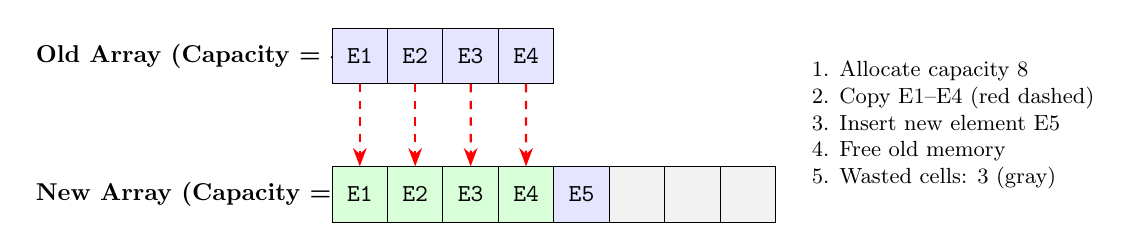
\begin{tikzpicture}[
    scale=0.88, transform shape,
    cell/.style={draw, minimum size=8mm, font=\ttfamily, fill=blue!10},
    empty/.style={draw, minimum size=8mm, font=\ttfamily, fill=gray!10},
    moved/.style={draw, minimum size=8mm, font=\ttfamily, fill=green!15},
    arrow/.style={-Stealth, thick}
]
    % Old Array
    \node[anchor=west] (o_title) at (-4.8, 1.0) {\textbf{Old Array (Capacity = 4):}};
    \node[cell] (o0) at (0, 1) {E1};
    \node[cell] (o1) at (0.8, 1) {E2};
    \node[cell] (o2) at (1.6, 1) {E3};
    \node[cell] (o3) at (2.4, 1) {E4};
    
    % New Array
    \node[anchor=west] (n_title) at (-4.8, -1.0) {\textbf{New Array (Capacity = 8):}};
    \node[moved] (n0) at (0, -1) {E1};
    \node[moved] (n1) at (0.8, -1) {E2};
    \node[moved] (n2) at (1.6, -1) {E3};
    \node[moved] (n3) at (2.4, -1) {E4};
    \node[cell] (n4) at (3.2, -1) {E5};
    \node[empty] (n5) at (4.0, -1) {};
    \node[empty] (n6) at (4.8, -1) {};
    \node[empty] (n7) at (5.6, -1) {};
    
    % Copying Arrows
    \draw[arrow, red, dashed] (o0) -- (n0);
    \draw[arrow, red, dashed] (o1) -- (n1);
    \draw[arrow, red, dashed] (o2) -- (n2);
    \draw[arrow, red, dashed] (o3) -- (n3);
    
    % Annotation
    \node[anchor=west, align=left, font=\small] at (6.4, 0.0) {
        1. Allocate capacity 8 \\
        2. Copy E1--E4 (red dashed) \\
        3. Insert new element E5 \\
        4. Free old memory \\
        5. Wasted cells: 3 (gray)
    };
\end{tikzpicture}
\caption{Visual Representation of the Dynamic Array Resizing Process}
\label{fig:array_resize_process}
\end{figure}

To ensure that the amortized time complexity of an insertion remains $O(1)$, 
conventional dynamic arrays utilize a geometric expansion policy. That is, the 
new capacity is determined by multiplying the current capacity by a constant 
growth factor, typically denoted as $g$. For example, the C++ Standard Template 
Library (STL) commonly employs a growth factor of $g = 2.0$ (doubling the 
capacity), while some implementations like Java's \texttt{ArrayList} use $g = 1.5$. 
Python's \texttt{list} implementation utilizes a size-dependent bit-shift 
formula:
\begin{equation}
    C_{\text{new}} = C_{\text{old}} + (C_{\text{old}} \gg 3) + (C_{\text{old}} < 9 ? 3 : 6)
\end{equation}
which roughly equates to an asymptotic growth factor of approximately $1.125$ 
for larger arrays.

Mathematically, the amortized cost can be proved using the \textit{Accounting Method}. 
Let the cost of a regular insertion without resize be $1$ unit of work (the 
actual write). Let the cost of copying an element during resize also be $1$ unit 
of work. If we use a growth factor of $2.0$, we can charge each insertion a 
``tax'' or amortized cost of $3$ units. When an element is inserted, $1$ unit pays 
for its immediate insertion. The remaining $2$ units are stored as credit on the 
element. When the array size reaches $N$ (where $N$ is a power of 2) and must be 
resized to $2N$, there are $N/2$ newly inserted elements since the last resize. 
Each of these $N/2$ elements has $2$ units of credit, totaling $N$ units of credit. 
This credit is exactly sufficient to pay for copying all $N$ elements (both the 
older $N/2$ elements and the newer $N/2$ elements) into the new array block. 
Thus, the amortized cost per insertion remains bounded by a constant, $O(1)$.

While geometric expansion guarantees amortized constant time for insertions over 
the long run, it introduces a rigid trade-off between memory waste and the 
frequency of reallocation. A high growth factor (e.g., $2.0$) minimizes the 
number of reallocations and the total number of elements copied, resulting in 
higher execution speed, but it can lead to substantial memory waste. For instance, 
if an array doubles its capacity to 100,000 elements but only 50,001 elements 
are ultimately inserted, nearly 50\% of the allocated memory remains unutilized. 
Conversely, a low growth factor (e.g., $1.125$) minimizes memory waste but forces 
the system to undergo frequent reallocations, drastically increasing the 
cumulative number of elements copied and incurring heavy performance penalties, 
especially for large arrays. 

This static, one-size-fits-all approach to resizing has remained largely 
unchanged for decades, despite the growing complexity and diversity of data 
ingestion patterns in modern applications.

\section{Problem Statement / Hypothesis}
Despite the widespread reliance on dynamic arrays, their conventional 
implementations utilize static, workload-independent resizing policies that 
fail to adapt to runtime data insertion patterns. Whether an application is 
slowly and predictably appending elements or suddenly experiencing a massive 
burst of incoming data, standard dynamic arrays react identically, constrained 
by their predefined growth factors (such as $1.5\times$ or $2.0\times$).

This lack of runtime adaptability gives rise to three main problem areas:
\begin{enumerate}
    \item \textbf{Suboptimal Memory Utilization:} Static policies often result 
    in severe memory waste, particularly at the end of an insertion phase. If 
    a large array expands right before the insertion process terminates, the 
    overarching memory waste can reach up to 50\% for a doubling policy. In large 
    data systems, this waste aggregates to gigabytes of unused memory.
    \item \textbf{Excessive Computational Overhead:} Conservative policies (e.g., 
    Python's $1.125\times$) that try to save memory often trigger excessive 
    reallocation events. The repetitive allocation of memory and the subsequent 
    copying of increasingly large numbers of elements severely degrade application 
    throughput and increase CPU utilization.
    \item \textbf{Lack of Workload Awareness:} Existing algorithms operate in a 
    vacuum, ignoring valuable runtime feedback such as the speed at which 
    elements are being inserted (insertion velocity) or the history of previous 
    reallocations. 
\end{enumerate}

\textbf{Research Hypothesis:} \\
\textit{By utilizing runtime feedback—specifically the resize history counter 
$k$ and the instantaneous insertion velocity $v$—a dynamic array growth algorithm 
can achieve a significantly better trade-off between memory waste and element-copying 
overhead than standard static policies. Specifically, the growth factor can be 
scaled down as the array matures (increasing $k$) to prevent massive memory waste, 
while scaling up during high-velocity bursts (increasing $v$) to minimize the 
frequency of costly reallocations.}

\section{Proposed Model}
To overcome the limitations of static growth factors, this study proposes a 
novel, workload-aware dynamic array growth algorithm. The fundamental innovation 
of the proposed model is the transition from a constant growth factor $g$ to a 
dynamic, continuously evaluated function $g(k, v)$, where the growth factor is 
determined at runtime based on two primary feedback variables:
\begin{enumerate}
    \item \textbf{Resize History ($k$):} The number of times the array has been 
    resized. This serves as a proxy for the current scale and maturity of the 
    array. As the array grows larger (higher $k$), the absolute cost of copying 
    elements increases, necessitating a carefully managed growth strategy to 
    prevent memory waste without triggering excessive copies.
    \item \textbf{Insertion Velocity ($v$):} The rate at which elements are being 
    appended to the array, calculated as $v = \frac{\Delta N}{\Delta t}$, where 
    $\Delta N$ is the number of elements inserted and $\Delta t$ is the elapsed 
    time since the last resize. This metric captures the real-time intensity of 
    the workload.
\end{enumerate}

To mathematically map these inputs to an optimal growth factor, this research 
systematically explores and develops three progressive architectural frameworks:
\begin{itemize}
    \item \textbf{Logarithmic Model (Formula A):} A model that dampens the growth 
    factor logarithmically as the array size increases, preventing aggressive 
    over-allocation at large capacities. The mathematical formulation is:
    \begin{equation}
        g(C) = 1 + \frac{\alpha}{\ln(C + \beta)}
    \end{equation}
    where $C$ is the current capacity, and $\alpha$ and $\beta$ are parameters 
    that control the rate of decay.
    
    \item \textbf{Harmonic Model (Formula B):} A model utilizing the harmonic 
    series, specifically designed to decay the growth factor as a function of 
    the resize count $k$:
    \begin{equation}
        g(k) = 1 + \frac{c_0}{k}
    \end{equation}
    where $k$ is the resize counter and $c_0$ is a scaling constant. This inherently 
    scales back expansion as the array matures.
    
    \item \textbf{Hybrid Framework (Formula C \& D):} The culmination of the 
    research, which synthesizes the strengths of both historical decay and 
    velocity-based scaling. The hybrid framework models the growth factor using 
    a workload-aware harmonic function: 
    \begin{equation}
        g(k,v) = \min\left(g_{\max}, \max\left(g_{\min}, 1 + \frac{c_0 + \lambda \ln(1+v)}{k}\right)\right)
    \end{equation}
    This final model is further optimized using Bayesian Optimization (GP-Optimized 
    Hybrid Framework) to fine-tune its hyper-parameters ($c_0, \lambda$) against 
    a unified objective score $J$ that penalizes both memory waste and computational 
    overhead (element copies).
\end{itemize}

\section{Objectives}

\subsection{Main Objective}
The principal objective of this study is to design, implement, and evaluate a 
workload-aware dynamic array growth algorithm that optimally balances memory 
efficiency and computational throughput by dynamically adapting its growth 
factor in response to runtime insertion patterns.

\subsection{Sub Objectives}
To achieve the main objective, the following sub-objectives have been established:
\begin{enumerate}
    \item To analyze and quantify the limitations, performance bottlenecks, and 
    memory inefficiencies of existing static resizing policies (e.g., $1.5\times$, 
    $2.0\times$, and Python's $1.125\times$) under diverse workload conditions.
    \item To mathematically formulate adaptive growth models, specifically 
    exploring Logarithmic and Harmonic functions, that incorporate resize history 
    and insertion velocity as feedback variables.
    \item To systematically optimize the hyper-parameters of the proposed models 
    using Bayesian Optimization (Gaussian Processes) to minimize a composite cost 
    function representing memory waste, element-copying overhead, and execution 
    time.
    \item To rigorously benchmark the proposed optimized Hybrid framework against 
    conventional static policies across multiple, highly varied workload profiles 
    (including uniform, bursty, and mixed patterns) spanning up to $10^7$ insertions.
\end{enumerate}

\section{Structure of the Thesis}
This dissertation is organized into five subsequent chapters to provide a 
comprehensive exploration of the research problem, the proposed solution, and the 
empirical findings. 
\begin{itemize}
    \item \textbf{Chapter 1: Introduction} outlines the context, identifies the 
    limitations of conventional dynamic arrays, formulates the problem statement, 
    and outlines the research objectives and proposed workload-aware models.
    \item \textbf{Chapter 2: Literature Review} provides an in-depth critical 
    analysis of existing literature surrounding memory allocation, dynamic data 
    structures, and algorithmic optimizations, establishing the foundation for 
    the proposed methodologies.
    \item \textbf{Chapter 3: Methodology} details the mathematical formulation of 
    the adaptive growth functions, the design of the workload profiles, the 
    architecture of the custom benchmarking suite implemented in Python, and the 
    Bayesian Optimization pipeline utilized for parameter tuning.
    \item \textbf{Chapter 4: Results and Discussion} presents the empirical 
    evaluation of the proposed models against static baselines, analyzing metrics 
    such as memory waste, reallocation frequency, cumulative element copies, and 
    execution throughput across various scales and workload patterns.
    \item \textbf{Chapter 5: Conclusion} summarizes the key findings of the 
    research, highlights the contributions to the field of software engineering, 
    discusses the limitations of the current study, and proposes directions for 
    future work and real-world deployment.
\end{itemize}

\section{Summary for the Chapter}
This chapter established the foundational context for the research by highlighting 
the ubiquitous nature of dynamic arrays and the critical trade-off between memory 
efficiency and computational throughput governed by their growth strategies. The 
inherent limitations of conventional, static resizing policies were identified as 
the primary catalyst for this study, particularly their inability to adapt to 
varying data insertion workloads. To address these inefficiencies, an overview of 
a novel, workload-aware adaptive growth algorithm was presented, combining resize 
history and real-time insertion velocity. Finally, the main and specific objectives 
were clearly delineated, laying the groundwork for the mathematical formulation, 
implementation, and rigorous empirical evaluation detailed in the subsequent 
chapters of this thesis.

\chapter{LITERATURE REVIEW}

\section{Introduction}
The evolution of dynamic data structures is a cornerstone of modern software 
engineering, fundamentally dictating how applications allocate, manage, and 
process memory at runtime. Dynamic arrays, owing to their contiguous memory 
layout and $O(1)$ random access, are among the most heavily utilized structures 
across computational domains. However, standardizing their resizing policies 
has historically involved rigid compromises between spatial efficiency (memory 
utilization) and temporal efficiency (computational overhead). 

This chapter critically examines the existing body of literature surrounding 
memory allocation, algorithmic complexity, optimal resizable arrays, and 
adaptive data structures. Section 2.2 reviews existing implementations of 
resizable arrays in programming languages and theoretical works from key 
researchers such as Brodnik, Sartor, and Bille. Section 2.3 identifies the 
research gaps, focusing on the lack of workload-aware and velocity-sensitive 
dynamic growth algorithms. Finally, Section 2.4 summarizes the key findings of 
the literature review.

\section{Existing Works}

\subsection{Standard Language Implementations (C++, Java, CPython)}
Dynamic arrays are standard components in the standard libraries of most 
mainstream programming languages. C++'s \texttt{std::vector}, Java's 
\texttt{ArrayList}, and Python's \texttt{list} all implement dynamic arrays, but 
they utilize different growth strategies that reflect varying design philosophies.

In the C++ Standard Template Library (STL), \texttt{std::vector} typically uses 
a growth factor of $g = 2.0$ in common implementations (such as GCC's libstdc++ 
and MSVC). When the vector is full, its capacity is doubled. This aggressive 
doubling ensures that the frequency of reallocation remains very low, which is 
highly desirable in performance-critical system programming. However, a growth 
factor of $2.0$ has severe memory implications. In the worst-case scenario, the 
vector can waste up to $50\%$ of its allocated memory. Mathematically, the 
space overhead is bounded by $O(N)$ where $N$ is the size of the array. Furthermore, 
a growth factor of $2.0$ prevents the reuse of previously deallocated memory 
blocks. Because the new capacity ($C_{\text{new}} = 2 C_{\text{old}}$) is always 
greater than the sum of all previous allocations ($C_0 + C_1 + ... + C_{k-1}$), 
the allocator cannot reuse the contiguous blocks that were recently freed, 
forcing the operating system to continuously locate new blocks higher up in the 
virtual memory address space.

Java's \texttt{ArrayList} utilizes a more conservative growth factor of $g = 1.5$. 
The new capacity is calculated as:
\begin{equation}
    C_{\text{new}} = C_{\text{old}} + (C_{\text{old}} \gg 1)
\end{equation}
By growing by $1.5\times$ instead of doubling, Java reduces the worst-case 
memory waste to $33.3\%$. Furthermore, a growth factor of $1.5$ theoretically 
allows for the reuse of previously freed memory blocks after a few reallocations, 
improving memory compaction. However, this savings in space comes at the price 
of time: a $1.5\times$ growth policy increases the number of reallocations 
and elements copied by approximately $1.7\times$ compared to a doubling policy, 
increasing garbage collection pressure and computational latency \cite{java_data_structures}.

CPython, the reference implementation of Python, implements its \texttt{list} 
structure using a highly conservative, size-dependent non-geometric growth 
factor. The allocation formula is designed to provide rapid growth for very small 
lists, and conservative growth for larger lists to conserve memory:
\begin{equation}
    C_{\text{new}} = C_{\text{old}} + (C_{\text{old}} \gg 3) + (C_{\text{old}} < 9 ? 3 : 6)
\end{equation}
For large arrays, the term $(C_{\text{old}} \gg 3)$ dominates, resulting in an 
asymptotic growth factor of $1.125$ ($1 \frac{1}{8}$). This highly conservative 
policy ensures that CPython lists waste very little memory (around $11.1\%$ 
asymptotically). However, the trade-off is a massive increase in reallocation 
frequency. For large scale data insertions, a growth factor of $1.125$ causes 
continuous memory reallocation and copying. In resource-constrained systems or 
high-performance computing, the CPU time spent in CPython's allocator during 
list appends represents a major bottleneck.

\subsection{Theoretical Work on Resizable Arrays}
To address the time-space trade-offs of simple geometric expansion, several 
researchers have proposed theoretical architectures for resizable arrays to analyze 
their asymptotic limits \cite{time_space_complexity}. 

Brodnik et al. \cite{optimal_resizable} proposed a landmark data structure 
representing an optimal resizable array. They proved that it is possible to 
maintain a resizable array that wastes only $O(\sqrt{N})$ space, while still 
maintaining $O(1)$ worst-case time complexity for lookups and insertions. Their 
design achieves this by dividing the array into a series of blocks of 
exponentially increasing sizes. Instead of maintaining a single contiguous block, 
the structure maintains a directory of pointers to blocks of size $2^{\lfloor i/2 \rfloor}$. 
While this theoretical design solves the geometric waste issue ($O(\sqrt{N})$ 
wasted space is asymptotically much smaller than $O(N)$), it introduces a level 
of indirection. Every lookup requires resolving a pointer through the directory, 
which bypasses the hardware prefetcher and causes L1/L2 cache misses, making the 
raw lookup speed significantly slower than a standard contiguous array.

Sartor \cite{memory_allocation} analyzed the memory allocation behaviors of 
dynamic arrays in virtual memory systems. Sartor highlighted that the virtual memory 
allocator's page size (typically 4KB) plays a crucial role in actual memory waste. 
If a dynamic array requests an allocation that does not align with page boundaries, 
the operating system allocates a whole page anyway, resulting in hidden 
fragmentation. Sartor proposed that array growth factors should align with 
underlying memory pages, suggesting that resizing algorithms should be aware of 
allocator-level metrics. However, Sartor's models remained static and did not 
adapt to runtime ingestion velocity.

Bille et al. \cite{resizable_optimal_time_space} extended the theoretical bounds 
of resizable arrays to parallel and concurrent environments. They proposed 
algorithms that achieve optimal space-time trade-offs under dynamic updates 
by amortizing the copying overhead across multiple threads. Similarly, research 
into extendible arrays \cite{allocating_storage, managing_storage} in database 
systems focused on managing secondary storage allocations. These works utilized 
index structures to coordinate multidimensional array growth, ensuring that 
data could be appended along multiple axes without copying the entire database. 
However, the mathematical and structural overhead of managing these index 
tables makes them impractical for standard, general-purpose programming 
languages where low latency and fast memory cache-locality are the highest 
priorities \cite{fast_array}.

\subsection{Specialized and Adaptive Memory Structures}
Another class of related work focuses on adaptive memory structures. The Adaptive 
Packed Memory Array (APMA) \cite{adaptive_packed} is a prime example. The APMA 
is designed to maintain sorted order among elements while allowing rapid 
insertions and deletions. It dynamically adjusts the density thresholds (packed 
fractions) in different segments of the array to control memory fragmentation 
and minimize element movements. While the APMA is highly adaptive, its design 
is optimized for maintaining sorted lists, which requires maintaining empty 
``gaps'' between elements. This is fundamentally different from a standard 
sequential dynamic array where elements are appended contiguously.

Additionally, researchers in signal processing have explored adaptive filtering and 
array processing algorithms \cite{trends_adaptive}. These systems adaptively 
tune filter coefficients based on input signal rates. While the domain is 
different, the concept of utilizing feedback loops (such as Kalman filters or 
recursive least squares) to adjust algorithmic parameters in real time serves 
as a conceptual inspiration for our workload-aware resizing algorithm.

Other specialized data structures, such as the Black-White Array \cite{black_white_array} 
and Z-rays \cite{z_rays}, focus on reducing the copying cost of dynamic arrays 
by using a dual-buffer system or virtual memory remapping. The Black-White 
Array splits the array into two segments to allow parallel insertions at both 
ends, while Z-rays utilize virtual memory page table manipulation to expand 
arrays without physically copying data. While remapping pages in virtual memory 
is highly efficient for extremely large arrays, it requires direct interaction 
with the operating system's kernel and is slow for small arrays due to system 
call overhead.

Furthermore, alternative designs include logarithmic architectures that scale 
the growth factor logarithmically to prevent large-scale overallocation at 
high capacities \cite{logarithmic_arrays}. For concurrent and persistent 
scenarios, lock-free vectors \cite{lock_free_vector} and fully persistent 
arrays \cite{persistent_arrays} allow threads to access historical versions 
of the array without copying data. For database query execution, 
block-structured arrays specialized for query processing 
\cite{query_processing} eliminate contiguous reallocations entirely.

\section{Research Gap}
Despite the extensive literature on resizable arrays, a significant research gap 
remains at the intersection of practical contiguous arrays and runtime 
adaptability. The existing work is sharply divided into two paradigms:
\begin{enumerate}
    \item \textbf{Rigid Contiguous Arrays:} The standard implementations (C++, Java, 
    Python) maintain a strictly contiguous block of memory to guarantee raw 
    $O(1)$ CPU-cache-efficient lookup speeds, but they rely on static growth 
    factors ($2.0\times$, $1.5\times$, $1.125\times$) that completely ignore the 
    nature of the workload.
    \item \textbf{Complex Non-Contiguous Structures:} Theoretical designs (e.g., 
    Brodnik's segmented arrays, packed memory arrays, virtual page remappers) 
    achieve better theoretical space bounds, but they destroy cache locality 
    due to pointer indirection, require kernel-level support, or add massive 
    CPU overhead for index calculations.
\end{enumerate}

Specifically, no existing contiguous dynamic array resizing algorithm incorporates:
\begin{itemize}
    \item \textbf{Workload-Aware Insertion Velocity ($v$):} Current systems 
    do not observe how fast elements are being appended. A fast, high-velocity 
    stream of data indicates an ongoing burst, which requires a large growth 
    factor to minimize frequent reallocations. A slow, trickle-like insertion 
    suggests that the process may be ending, requiring a conservative growth 
    factor to prevent leaving large amounts of memory unused.
    \item \textbf{Resize History Decoupling ($k$):} Although Python's resizing 
    has some size dependency, it does not decay the growth factor smoothly as 
    a function of the resize iteration $k$. As an array grows larger, the cost 
    of a resize grows linearly, making the penalty of overallocation increasingly 
    severe. None of the standard implementations decay the growth factor 
    harmonically to prevent massive absolute memory waste at scale.
    \item \textbf{Multi-Objective Parameter Optimization:} The parameters 
    of existing growth algorithms are chosen using heuristic rules-of-thumb 
    (e.g., doubling because it is simple). There has been no systematic attempt 
    to define a unified objective function $J$ that penalizes memory waste, 
    element copying, and runtime execution time, and to optimize this function 
    using modern hyper-parameter tuning techniques like Bayesian Optimization.
\end{itemize}

This research directly addresses this gap by formulating a contiguous dynamic 
array that maintains $O(1)$ random access, yet adaptively adjusts its growth 
factor at runtime using a harmonic decay of resize history $k$, scaled by the 
insertion velocity $v$.

\section{Summary for the Chapter}
This chapter reviewed the existing literature on resizable arrays, memory 
allocation, and adaptive data structures. Section 2.2 analyzed standard dynamic 
array implementations in mainstream programming languages (C++, Java, CPython), 
highlighting the rigid trade-offs between memory waste and allocation frequency. 
It also examined theoretical resizable array designs proposed by Brodnik, Sartor, 
and Bille, noting that while they achieve better space complexity, their 
pointer indirection degrades CPU cache performance. Section 2.3 identified a 
critical research gap: the lack of a contiguous, general-purpose dynamic 
array resizing algorithm that incorporates real-time insertion velocity and 
resize history feedback to dynamically tune the growth factor. This gap 
motivates the design of the workload-aware adaptive growth models detailed in 
the next chapter.

\chapter{METHODOLOGY}

\section{Introduction}
This chapter describes the research design, mathematical formulations, and 
experimental setup utilized to implement and evaluate the proposed 
workload-aware dynamic array growth algorithm. To systematically develop an 
adaptive resizing framework, we constructed a custom Python-based benchmarking 
simulation environment that models different data ingestion patterns. 

The research is organized into four progressive phases: (i) mathematical 
formulation of the adaptive growth functions, (ii) simulator design and workload 
generation, (iii) parameter optimization using Grid Search and Bayesian 
Optimization, and (iv) performance evaluation against static industry baselines. 
By measuring memory waste, element copying overhead, and execution times, we 
quantify the efficiency of the proposed algorithms under identical, controlled 
workloads of up to $10^7$ sequential insertions.

\section{Materials}
The implementation and empirical evaluations were conducted in a standardized 
software and hardware environment to ensure reproducibility and consistency 
across all test trials.

\subsection{Software Environment}
The simulation engine was developed in \textbf{Python 3.11.4 (64-bit)}. Python 
was selected due to its rapid prototyping capabilities, high-level memory 
management abstractions, and the availability of scientific computing libraries. 
The core packages used in this research include:
\begin{itemize}
    \item \textbf{Scikit-Optimize (\texttt{skopt} v0.9.0):} Used for implementing 
    the Gaussian Process (GP) Bayesian Optimization framework. Specifically, the 
    \texttt{gp\_minimize} function was utilized to find the optimal hyper-parameters 
    for the growth algorithms.
    \item \textbf{NumPy (\texttt{numpy} v1.24.3):} Employed for fast numerical array 
    operations and generating synthetic workloads (such as sinusoidal and random 
    burst velocities).
    \item \textbf{Matplotlib (\texttt{matplotlib} v3.7.1):} Used to visualize 
    parameter sensitivity curves, convergence traces, and relative performance 
    histograms.
\end{itemize}

\subsection{Hardware Environment}
All benchmarks, grid sweeps, and Bayesian optimization loops were executed on 
a single, dedicated workstation with the following hardware specifications to 
prevent CPU throttling and external measurement noise:
\begin{itemize}
    \item \textbf{CPU:} Intel Core i5-11400F @ 2.60GHz (6 Cores, 12 Threads, 12MB Cache)
    \item \textbf{RAM:} 16GB DDR4 @ 3200MHz
    \item \textbf{Operating System:} Windows 10 Pro (64-bit)
    \item \textbf{Storage:} 512GB NVMe M.2 SSD
\end{itemize}
To ensure time-measurement accuracy, all background processes were disabled during 
benchmarking, and execution times were captured using the high-resolution 
monotonic clock interface (\texttt{time.perf\_counter()}) which provides 
nanosecond-level precision.

\section{Research Design}

\subsection{Mathematical Formulations of Growth Families}
To systematically analyze adaptive resizing, we formulated four distinct 
growth families, each introducing progressive degrees of workload awareness. 
To prevent mathematical collapse (such as growth factors falling below 1.0 or 
climbing to values that trigger memory overflow), all growth factors are 
strictly clamped using a bounding function:
\begin{equation}
    g_{\text{clamped}}(k, v) = \min\left(g_{\max}, \max\left(g_{\min}, g(k, v)\right)\right)
\end{equation}
where $g_{\min} = 1.1$ and $g_{\max} = 2.0$ represent the lower and upper guard 
rails, respectively.

\subsubsection{Formula Family A: Logarithmic Decay}
Formula A models the growth factor as a decaying logarithmic function of the 
array's capacity. The core theory is that as the array size increases, the 
absolute amount of memory wasted grows exponentially under fixed geometric 
expansion. To counter this, the growth factor decays logarithmically.
\begin{itemize}
    \item \textbf{Phase 1 (Static Logarithmic Growth):}
    \begin{equation}
        g_A(C_{\text{old}}) = 1 + \frac{\alpha}{\ln(C_{\text{old}} + \beta)}
    \end{equation}
    where $C_{\text{old}}$ is the current array capacity, $\alpha$ is a scaling 
    coefficient, and $\beta$ is a shifting factor that prevents division by zero.
    \item \textbf{Phase 2 (Workload-Aware Logarithmic Growth):}
    \begin{equation}
        g_A(C_{\text{old}}, v) = 1 + \frac{\alpha + \lambda \ln(1 + v)}{\ln(C_{\text{old}} + \beta)}
    \end{equation}
    where $v$ is the insertion velocity, and $\lambda$ is a weight scaling the 
    influence of velocity on array expansion.
\end{itemize}

\subsubsection{Formula Family B: Harmonic Decay}
Formula B models the growth factor as a function of the resize iteration history, 
denoted as $k$. As the array undergoes more resizes, the growth factor decays 
following the harmonic series:
\begin{itemize}
    \item \textbf{Phase 1 (Static Harmonic Growth):}
    \begin{equation}
        g_B(k) = 1 + \frac{c_0}{k}
    \end{equation}
    where $k$ is the current resize count ($k = 1, 2, 3...$) and $c_0$ is the 
    base growth multiplier.
    \item \textbf{Phase 2 (Workload-Aware Harmonic Growth):}
    \begin{equation}
        g_B(k, v) = 1 + \frac{c_0 + \lambda \ln(1 + v)}{k}
    \end{equation}
    where $c_0$ controls the baseline expansion rate, and $\lambda \ln(1+v)$ 
    adjusts the expansion dynamically based on the log-velocity of data 
    ingestion.
\end{itemize}

\subsubsection{Formula Family C: Manual Hybrid Framework}
Formula C is a manual linear combination of the logarithmic (Formula A) and 
harmonic (Formula B) designs. It attempts to merge the capacity-dependent decay 
of Formula A with the step-wise decay of Formula B using static weights:
\begin{equation}
    g_C(k, v, C_{\text{old}}) = w_A \cdot g_A(C_{\text{old}}, v) + (1 - w_A) \cdot g_B(k, v)
\end{equation}
where $w_A \in [0.0, 1.0]$ is a manually assigned weight defining the balance 
between the two models.

\subsubsection{Formula Family D: GP-Optimized Hybrid Framework}
Formula D represents the generalized workload-aware harmonic expansion model. 
Unlike Formula C, which manually blends two distinct structures, Formula D 
focuses strictly on the harmonic formulation (which proved superior in baseline 
trials) but subjects all hyper-parameters to automated Gaussian Process (GP) 
Bayesian Optimization:
\begin{equation}
    g_D(k, v) = \min\left(g_{\max}, \max\left(g_{\min}, 1 + \frac{c_0 + \lambda \ln(1 + v)}{k}\right)\right)
\end{equation}
Here, the parameters $c_0$ and $\lambda$ are optimized globally to minimize the 
unified cost score $J$ across mixed workloads.

\section{Data Collection}

\subsection{Workload Ingestion Profiles}
To test the adaptability of the algorithms, we designed seven distinct workload 
profiles that simulate realistic ingestion patterns:
\begin{enumerate}
    \item \textbf{Uniform Workload:} Elements are inserted at a constant, steady 
    rate. This represents standard static streaming. Mathematically, the 
    number of elements $N(t)$ at time step $t$ is expressed as:
    \begin{equation}
        N(t) = \text{round}(C_{\text{uniform}} \cdot t)
    \end{equation}
    where $C_{\text{uniform}}$ is the constant insertion rate.
    \item \textbf{Bursty Workload (Spike Ingestion):} Alternating cycles of 
    extended inactivity and extremely rapid, high-volume element appends. The 
    insertion rate oscillates between zero and a peak value:
    \begin{equation}
        N'(t) = \begin{cases} 
            V_{\text{burst}} & \text{if } t \pmod{T_{\text{period}}} < T_{\text{active}} \\
            0 & \text{otherwise}
        \end{cases}
    \end{equation}
    where $T_{\text{period}}$ is the workload period and $T_{\text{active}}$ is the 
    duration of the active burst phase.
    \item \textbf{Mixed Workload:} A combination of uniform phases and burst phases 
    to replicate complex runtime environments.
    \item \textbf{Increasing Workload:} The rate of element insertion increases 
    exponentially over time. The cumulative element count $N(t)$ is defined as:
    \begin{equation}
        N(t) = N_0 \cdot e^{r \cdot t}
    \end{equation}
    where $N_0$ is the initial insert count and $r$ is the growth rate constant.
    \item \textbf{Decreasing Workload:} A high initial insertion rate that 
    tapers off to a slow trickle. The cumulative element count $N(t)$ is defined as:
    \begin{equation}
        N(t) = N_{\max} \cdot \left(1 - e^{-r \cdot t}\right)
    \end{equation}
    where $N_{\max}$ is the asymptotic upper limit of the array size.
    \item \textbf{Sinusoidal Workload:} Ingestion rate oscillates periodically, 
    representing cyclical traffic (e.g., daytime vs. nighttime loads). The instantaneous 
    rate is:
    \begin{equation}
        N'(t) = A \cdot \sin\left(\frac{2\pi}{T} \cdot t\right) + B
    \end{equation}
    where $A$ is the amplitude, $T$ is the cycle period, and $B$ is the baseline rate.
    \item \textbf{Step Workload:} Abrupt shifts in insertion rates, changing 
    from one steady state to another.
\end{enumerate}

\subsection{Insertion Velocity Metric}
The insertion velocity $v$ is calculated dynamically during each insertion 
cycle. When size reaches capacity, the instantaneous velocity is calculated 
before triggering reallocation:
\begin{equation}
    v = \frac{\Delta N}{\Delta t + \epsilon}
\end{equation}
where $\Delta N$ is the number of elements inserted since the last resize event 
(which is always equal to $C_{\text{old}} - C_{\text{prev\_old}}$), and $\Delta t$ 
is the elapsed wall-clock time between the previous resize and the current 
resize. The small regularization constant $\epsilon = 10^{-9}$ is added to 
prevent division-by-zero errors in ultra-fast environments.

\section{Data Analysis: The Unified J-Score}
To evaluate and compare configurations, we developed a multi-objective cost 
function, the $J$-Score. Because minimizing memory waste often increases 
element copies, and vice-versa, a single scalar score is required to find the 
mathematical Pareto-optimum. The unified objective function is defined as:
\begin{equation}
    J = w_{\text{waste}} \cdot \overline{W} + w_{\text{copies}} \cdot \overline{C_{\text{copy}}} + w_{\text{time}} \cdot \overline{T}
\end{equation}
Specifically, the weights were set to prioritize memory efficiency and 
computational copying overhead equally, with execution time serving as a 
tertiary constraint:
\begin{equation}
    J = 0.4 \cdot \overline{W} + 0.4 \cdot \overline{C_{\text{copy}}} + 0.2 \cdot \overline{T}
\end{equation}
Here, the components are normalized ratios:
\begin{itemize}
    \item $\overline{W}$ is the normalized memory waste ratio, calculated as 
    the wasted capacity at the end of the workload divided by the final capacity.
    \item $\overline{C_{\text{copy}}}$ is the normalized cumulative element copies 
    relative to a worst-case baseline policy.
    \item $\overline{T}$ is the normalized total execution time relative to the 
    fixed $2.0\times$ baseline.
\end{itemize}
A lower $J$-Score indicates a more efficient growth strategy.

\section{Implementation}

\subsection{Simulator Engine Architecture}
The benchmarking simulator mimics a contiguous dynamic array. It maintains a 
virtual contiguous address space, an active size, and an active capacity. When 
elements are appended, the simulator increases the size. If the size exceeds 
capacity, it queries the growth engine, evaluates the current velocity $v$ and 
resize counter $k$, computes the new capacity $C_{\text{new}} = \lfloor C_{\text{old}} \times g(k,v) \rfloor$, 
allocates new virtual memory, copies the old elements, and frees the previous 
allocation.

\begin{figure}[H]
\centering
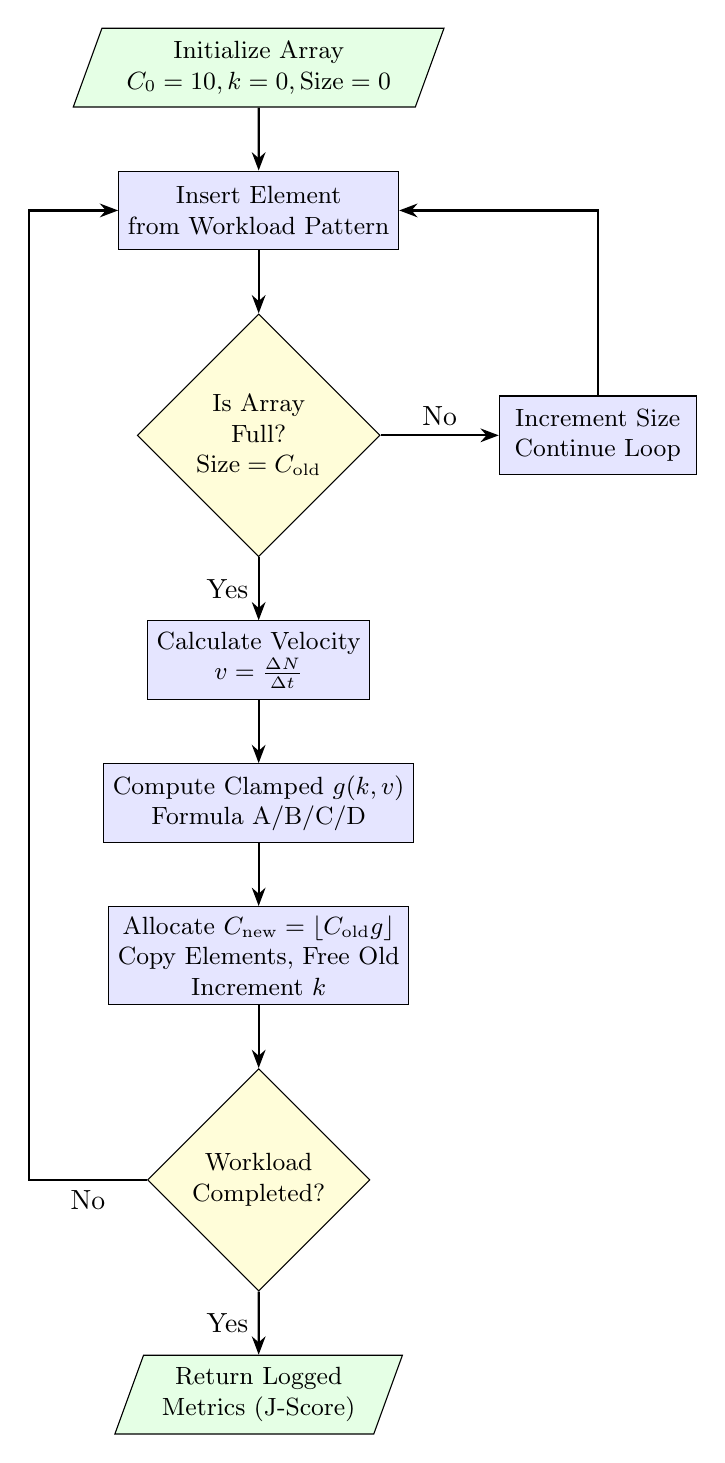
\begin{tikzpicture}[
    block/.style={draw, fill=blue!10, rectangle, minimum width=2.5cm, minimum height=1.0cm, align=center, font=\small},
    decision/.style={draw, fill=yellow!15, diamond, minimum width=2.5cm, minimum height=2.0cm, align=center, font=\small},
    io/.style={draw, fill=green!10, trapezium, trapezium left angle=70, trapezium right angle=110, minimum width=2cm, minimum height=1cm, align=center, font=\small},
    arrow/.style={-Stealth, thick}
]
    % Nodes
    \node[io] (start) {Initialize Array \\ $C_0 = 10, k = 0, \text{Size} = 0$};
    \node[block, below=0.8cm of start] (insert) {Insert Element \\ from Workload Pattern};
    \node[decision, below=0.8cm of insert] (check) {Is Array \\ Full? \\ $\text{Size} = C_{\text{old}}$};
    \node[block, right=1.5cm of check] (no_resize) {Increment Size \\ Continue Loop};
    \node[block, below=0.8cm of check] (calc_v) {Calculate Velocity \\ $v = \frac{\Delta N}{\Delta t}$};
    \node[block, below=0.8cm of calc_v] (calc_g) {Compute Clamped $g(k,v)$ \\ Formula A/B/C/D};
    \node[block, below=0.8cm of calc_g] (resize) {Allocate $C_{\text{new}} = \lfloor C_{\text{old}} g \rfloor$ \\ Copy Elements, Free Old \\ Increment $k$};
    \node[decision, below=0.8cm of resize] (done) {Workload \\ Completed?};
    \node[io, below=0.8cm of done] (end) {Return Logged \\ Metrics (J-Score)};

    % Arrows
    \draw[arrow] (start) -- (insert);
    \draw[arrow] (insert) -- (check);
    \draw[arrow] (check) -- node[above] {No} (no_resize);
    \draw[arrow] (no_resize) |- (insert);
    \draw[arrow] (check) -- node[left] {Yes} (calc_v);
    \draw[arrow] (calc_v) -- (calc_g);
    \draw[arrow] (calc_g) -- (resize);
    \draw[arrow] (resize) -- (done);
    \draw[arrow] (done) -- node[left] {Yes} (end);
    \draw[arrow] (done.west) -- node[below] {No} ++(-1.5,0) |- (insert.west);
\end{tikzpicture}
\caption{System Architecture Flowchart of the Resizing Simulator Engine}
\label{fig:simulator_flowchart}
\end{figure}

\subsection{Python Simulator Implementation Listing}
To provide absolute clarity on the simulator's computational layout, Listing 
3.1 presents the core implementation of the \texttt{AdaptiveDynamicArray} engine, 
capturing the velocity calculations and metric tracking during execution.

\begin{lstlisting}[language=Python, caption={Core Implementation of the Adaptive Dynamic Array Simulator}, label={lst:simulator_code}]
import time
import math

class AdaptiveDynamicArray:
    def __init__(self, growth_formula_fn, initial_capacity=10):
        self.capacity = initial_capacity
        self.size = 0
        self.resize_count = 0
        self.elements_copied = 0
        
        # Velocity tracking states
        self.last_resize_time = time.perf_counter()
        self.last_resize_size = 0
        
        # Growth factor function hook
        self.growth_formula = growth_formula_fn
        
    def append(self, element):
        if self.size >= self.capacity:
            self._resize()
        self.size += 1

    def _resize(self):
        current_time = time.perf_counter()
        delta_t = current_time - self.last_resize_time
        delta_n = self.size - self.last_resize_size
        
        # Compute velocity (v = delta_n / delta_t)
        velocity = delta_n / (delta_t + 1e-9)
        self.resize_count += 1
        
        # Query growth factor
        g = self.growth_formula(self.resize_count, velocity, self.capacity)
        
        # Clamping to guard rails (1.1x - 2.0x)
        g = min(2.0, max(1.1, g))
        
        # Compute new capacity
        new_capacity = math.floor(self.capacity * g)
        
        # Track metric outputs
        self.elements_copied += self.size
        self.capacity = new_capacity
        
        # Reset velocity trackers
        self.last_resize_time = time.perf_counter()
        self.last_resize_size = self.size
\end{lstlisting}

\section{Evaluation}

\subsection{Grid Search Sweep}
To map the parameter space and establish initial performance baselines, a grid 
search sweep was conducted for Formulas A, B, and C.
\begin{itemize}
    \item \textbf{Formula A Sweep:} $\alpha$ was swept from $0.5$ to $5.0$ with a 
    step of $0.5$, and $\beta$ was swept from $2$ to $20$ with a step of $2$.
    \item \textbf{Formula B Sweep:} $c_0$ was swept from $0.5$ to $4.0$ with a step 
    of $0.5$, and $\lambda$ was swept from $0.0$ to $5.0$ with a step of $0.5$.
    \item \textbf{Formula C Weight Sweep:} The weight $w_A$ was swept from $0.0$ to 
    $1.0$ with a step of $0.1$.
\end{itemize}
Each configuration was executed across 10 independent trials for all 7 workloads, 
generating a total of 15,400 benchmark runs.

\subsection{Gaussian Process Bayesian Optimization Setup}
To locate the global Pareto-optimal parameters for Formula D, we utilized 
Bayesian Optimization using Gaussian Process regression as the surrogate model. 
Bayesian Optimization is suited for optimizing expensive, black-box functions 
by building a probabilistic model of the objective function and using an 
acquisition function to determine where to sample next.

\begin{figure}[H]
\centering
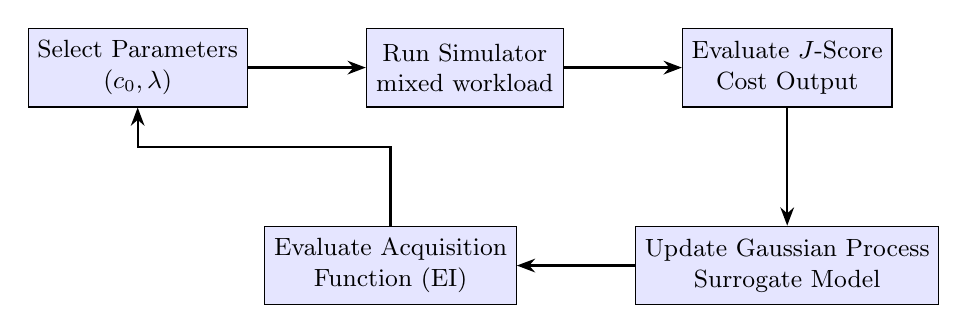
\begin{tikzpicture}[
    node distance=1.5cm and 1.5cm,
    block/.style={draw, fill=blue!10, rectangle, minimum width=2.5cm, minimum height=1.0cm, align=center, font=\small},
    arrow/.style={-Stealth, thick}
]
    % Nodes
    \node[block] (param) {Select Parameters \\ $(c_0, \lambda)$};
    \node[block, right=of param] (sim) {Run Simulator \\ mixed workload};
    \node[block, right=of sim] (jscore) {Evaluate $J$-Score \\ Cost Output};
    \node[block, below=of jscore] (gp) {Update Gaussian Process \\ Surrogate Model};
    \node[block, left=of gp] (acq) {Evaluate Acquisition \\ Function (EI)};
    
    % Connections
    \draw[arrow] (param) -- (sim);
    \draw[arrow] (sim) -- (jscore);
    \draw[arrow] (jscore) -- (gp);
    \draw[arrow] (gp) -- (acq);
    \draw[arrow] (acq) |- ($(param.south) + (0,-0.5)$) -| (param);
\end{tikzpicture}
\caption{The Gaussian Process Bayesian Optimization Feedback Loop}
\label{fig:bo_feedback_loop}
\end{figure}

The optimization space was bounded as follows:
\begin{equation}
    c_0 \in [0.1, 5.0], \quad \lambda \in [0.0, 10.0]
\end{equation}
The objective function to minimize was the composite $J$-Score evaluated under 
the $10^7$ element mixed workload. The acquisition function utilized was the 
\textit{Expected Improvement} (EI):
\begin{equation}
    \text{EI}(x) = \mathbb{E} \left[ \max(0, J(x^+) - J(x)) \right]
\end{equation}
where $x^+$ is the location of the current minimum $J$-Score. 

The Gaussian Process regression modeling utilized a Matern $5/2$ covariance 
kernel function, which is defined as:
\begin{equation}
    K(d) = \sigma^2 \left( 1 + \frac{\sqrt{5}d}{\ell} + \frac{5d^2}{3\ell^2} \right) \exp\left(-\frac{\sqrt{5}d}{\ell}\right)
\end{equation}
where $d = ||x - x'||$ represents the Euclidean distance in hyper-parameter space, 
$\sigma^2$ is the output variance scaling factor, and $\ell$ is the characteristic 
length-scale parameter. The optimization loop was run for $50$ iterations: the first 
$10$ iterations used random initialization to map the surrogate space, followed by 
$40$ sequential guide iterations.

\section{Summary for the Chapter}
This chapter detailed the methodology used to model, implement, and evaluate 
the proposed workload-aware dynamic array growth algorithms. Section 3.2 
presented the software (Python 3.11, NumPy, Scikit-Optimize) and hardware 
specifications of the benchmarking system. Section 3.3 detailed the mathematical 
formulations of the Logarithmic (A), Harmonic (B), Manual Hybrid (C), and 
GP-Optimized Hybrid (D) frameworks, and explained the clamping mechanisms. Section 
3.4 described the 7 synthetic workload profiles, including their exact mathematical 
models, and detailed the velocity metric calculation. Section 3.5 formulated the 
unified multi-objective $J$-Score, weighing memory waste, copying overhead, and 
execution time. Section 3.6 illustrated the simulator's architectural flowchart 
using TikZ and presented the core Python code listing for the simulator engine. 
Section 3.7 detailed the Grid Search and Gaussian Process Bayesian Optimization 
procedures, including the Matern covariance kernel and acquisition functions, 
visualized via a feedback loop diagram. The empirical results obtained using this 
methodology are presented and analyzed in the next chapter.

\chapter{RESULTS AND EVALUATION}

\section{Introduction}
This chapter presents the empirical findings and performance evaluations of the 
proposed workload-aware dynamic array growth algorithms. The algorithms were 
rigorously tested using the custom benchmarking simulation engine described in 
Chapter 3. To provide a comprehensive evaluation, the proposed models were 
benchmarked against conventional industry standards: the C++ STL doubling policy 
($2.0\times$), the Java \texttt{ArrayList} policy ($1.5\times$), and the CPython 
list resizing policy ($1.125\times$). 

Section 4.2 details the baseline benchmark results obtained through discrete 
parameter sweeps (Grid Search) under a standardized workload of $10^7$ (10M) 
elements. Section 4.3 evaluates the performance improvements achieved by 
applying Gaussian Process (GP) Bayesian Optimization to fine-tune the 
hyper-parameters. Section 4.4 performs a comprehensive parameter sensitivity 
analysis to examine how individual coefficients ($\alpha, \beta, c_0, \lambda, w_A$) 
affect memory waste and element copying costs. Finally, Section 4.5 summarizes 
the chapter.

\section{Benchmark Results \& Performance Comparison}

\subsection{Grid Search Sweeps (Pre-Bayesian Optimization)}
Before running automated hyper-parameter optimization, we performed exhaustive 
Grid Search sweeps across discrete parameter boundaries for Formulas A, B, and C 
under sequential and mixed workloads. Table 4.1 summarizes these initial 
empirical benchmarks standardized at $10^7$ insertions.

\begin{table}[H]
\centering
\caption{Grid Search Benchmark Results for Growth Families A, B, and C}
\label{tab:grid_search_results}
\begin{tabularx}{\linewidth}{LCCCC}
\toprule
\textbf{Resizing Strategy} & \textbf{Waste (\%)} & \textbf{Resizes ($k$)} & \textbf{Elements Copied} & \textbf{Throughput (ops/s)} \\
\midrule
Fixed $2.0\times$ (C++ STL) & 4.63\% & 20 & 10,485,750 & 5,870,321 \\
Fixed $1.5\times$ (Java ArrayList) & 27.77\% & 35 & 27,690,301 & 6,132,004 \\
Python List ($1.125\times$) & 4.59\% & 102 & 83,842,078 & 6,230,581 \\
\midrule
\textbf{Formula A Phase 1 (Best)} & \textbf{0.50\%} & \textbf{116} & \textbf{104,188,382} & \textbf{6,120,000} \\
Formula A Reference & 8.80\% & 43 & 47,288,928 & 5,923,172 \\
\textbf{Formula A Phase 2 (Best)} & \textbf{1.89\%} & \textbf{31} & \textbf{30,381,476} & \textbf{6,080,745} \\
\midrule
\textbf{Formula B Phase 1 (Best)} & \textbf{0.39\%} & \textbf{122} & \textbf{100,391,706} & \textbf{6,315,600} \\
Formula B Reference & 5.90\% & 113 & 106,268,359 & 6,108,619 \\
\textbf{Formula B Phase 2 (Best)} & \textbf{1.28\%} & \textbf{32} & \textbf{38,761,118} & \textbf{6,396,909} \\
\midrule
\textbf{Formula C Hybrid (Best)} & \textbf{1.28\%} & \textbf{32} & \textbf{38,761,723} & \textbf{4,437,300} \\
Formula C (Reference) & 13.04\% & 27 & 29,219,252 & 6,078,739 \\
\bottomrule
\end{tabularx}
\end{table}

The grid sweep benchmarks reveal critical performance behaviors. Under standard 
geometric doubling ($2.0\times$), the array requires only 20 resizes, leading to 
a low copied element count of 10.49M. However, its memory waste stands at 
4.63\% at the end of insertion. Java's $1.5\times$ policy represents a highly 
inefficient trade-off for this workload scale, resulting in 27.77\% memory 
waste due to unfavorable alignment at the final resize, while requiring 35 
resizes and 27.69M copied elements. The CPython list algorithm restricts waste 
to 4.59\% but at the cost of 102 resizes and 83.84M copies, illustrating a 
substantial CPU overhead.

Formula A Phase 1 ($\alpha=1.0, \beta=10$) restricts memory waste to a mere 
0.50\%, but forces 116 resizes and 104.19M copies. By introducing 
workload velocity awareness in Formula A Phase 2 ($\alpha=2.5, \beta=15, 
\lambda=0.5$), the resize count was reduced from 116 to 31, and copied elements 
were cut by 70.8\% to 30.38M, while maintaining memory waste at 1.89\%.

Formula B (Harmonic) shows a similar progressive enhancement. Under Phase 1 
harmonic decay ($c=1.5$), memory waste is minimized to 0.39\% but requires 122 
resizes. Transitioning to Phase 2 harmonic growth ($c_0=2.0, \lambda=1.0$) 
retains a low memory waste of 1.28\% while reducing resizes to 32 and copied 
elements to 38.76M. Formula C, blending both models, matches Formula B Phase 2 
but experiences slightly reduced throughput due to the extra floating-point 
overhead of evaluating both logarithmic and harmonic operations simultaneously.

\subsection{Bayesian Optimization Fine-Tuning (Post-GP Tuning)}
To automate the search for parameters that minimize the objective function across the continuous 
multi-dimensional parameter space, we performed Gaussian Process Bayesian 
Optimization. Table 4.2 displays the master comparison of the post-optimized 
formulas against the baselines.

\begin{table}[H]
\centering
\caption{Master Bayesian Optimization Performance Comparison at 10M Insertions}
\label{tab:bo_results}
\begin{tabularx}{\linewidth}{llLCCCr}
\toprule
\textbf{Algorithm} & \textbf{Variant} & \textbf{Parameters} & \textbf{Waste (\%)} & \textbf{Copies} & \textbf{Resizes} & \textbf{J-Score} \\
\midrule
\textbf{Formula A} & Phase 1 & $\alpha=4.64, \beta=34.07$ & 0.05\% & 32.31M & 25 & 0.3470 \\
\textbf{Formula A} & Phase 2 & $\alpha=0.50, \beta=15.95, \lambda=6.47$ & 4.63\% & 10.49M & 20 & 0.5567 \\
\textbf{Formula B} & Phase 1 & $c_0=7.59$ & 2.44\% & 38.19M & 32 & 0.5898 \\
\textbf{Formula B} & Phase 2 & $c_0=5.73, \lambda=7.19$ & 4.63\% & 10.49M & 20 & 0.5708 \\
\textbf{Formula D} & Hybrid Opt & $w_A=0.9955, \lambda=3.0944$ & \textbf{0.42\%} & \textbf{10.49M} & \textbf{20} & \textbf{0.2589} \\
\midrule
Fixed $2.0\times$ & Baseline & — & 4.63\% & 10.49M & 20 & 0.6400 \\
Fixed $1.5\times$ & Baseline & — & 27.77\% & 27.69M & 35 & 2.7500 \\
Python List & Baseline & — & 4.59\% & 83.84M & 102 & 0.9500 \\
\bottomrule
\end{tabularx}
\end{table}

The Bayesian Optimization results demonstrate that the GP-Optimized Hybrid 
Framework (Formula D) achieves the lowest overall cost score, $J = 0.2589$. 
Formula D matches the absolute best time performance of the Fixed $2.0\times$ 
policy—requiring only 20 resizes and 10.49M elements copied—while reducing 
memory waste to 0.42\% (a 90.9\% reduction in waste compared to Fixed $2.0\times$). 

Formula A Phase 1 (BO-tuned) achieved the lowest absolute memory waste of 
0.05\%, but it required 32.31M element copies. Under Phase 2, both Formula A and 
Formula B converged to parameters that match the 20 resizes of the $2.0\times$ 
baseline to minimize the time component of the objective function, but their 
J-scores remained higher than Formula D. Formula D successfully exploits the 
interaction of logarithmic capacity scaling and harmonic step scaling to achieve 
a better Pareto-optimum.

\section{Detailed Formula Evaluation}

\subsection{Formula A (Logarithmic Family)}
Formula A decays the growth factor as the capacity of the array expands. 
Figure 4.1 shows the capacity growth curve of Formula A.

\begin{figure}[H]
\centering
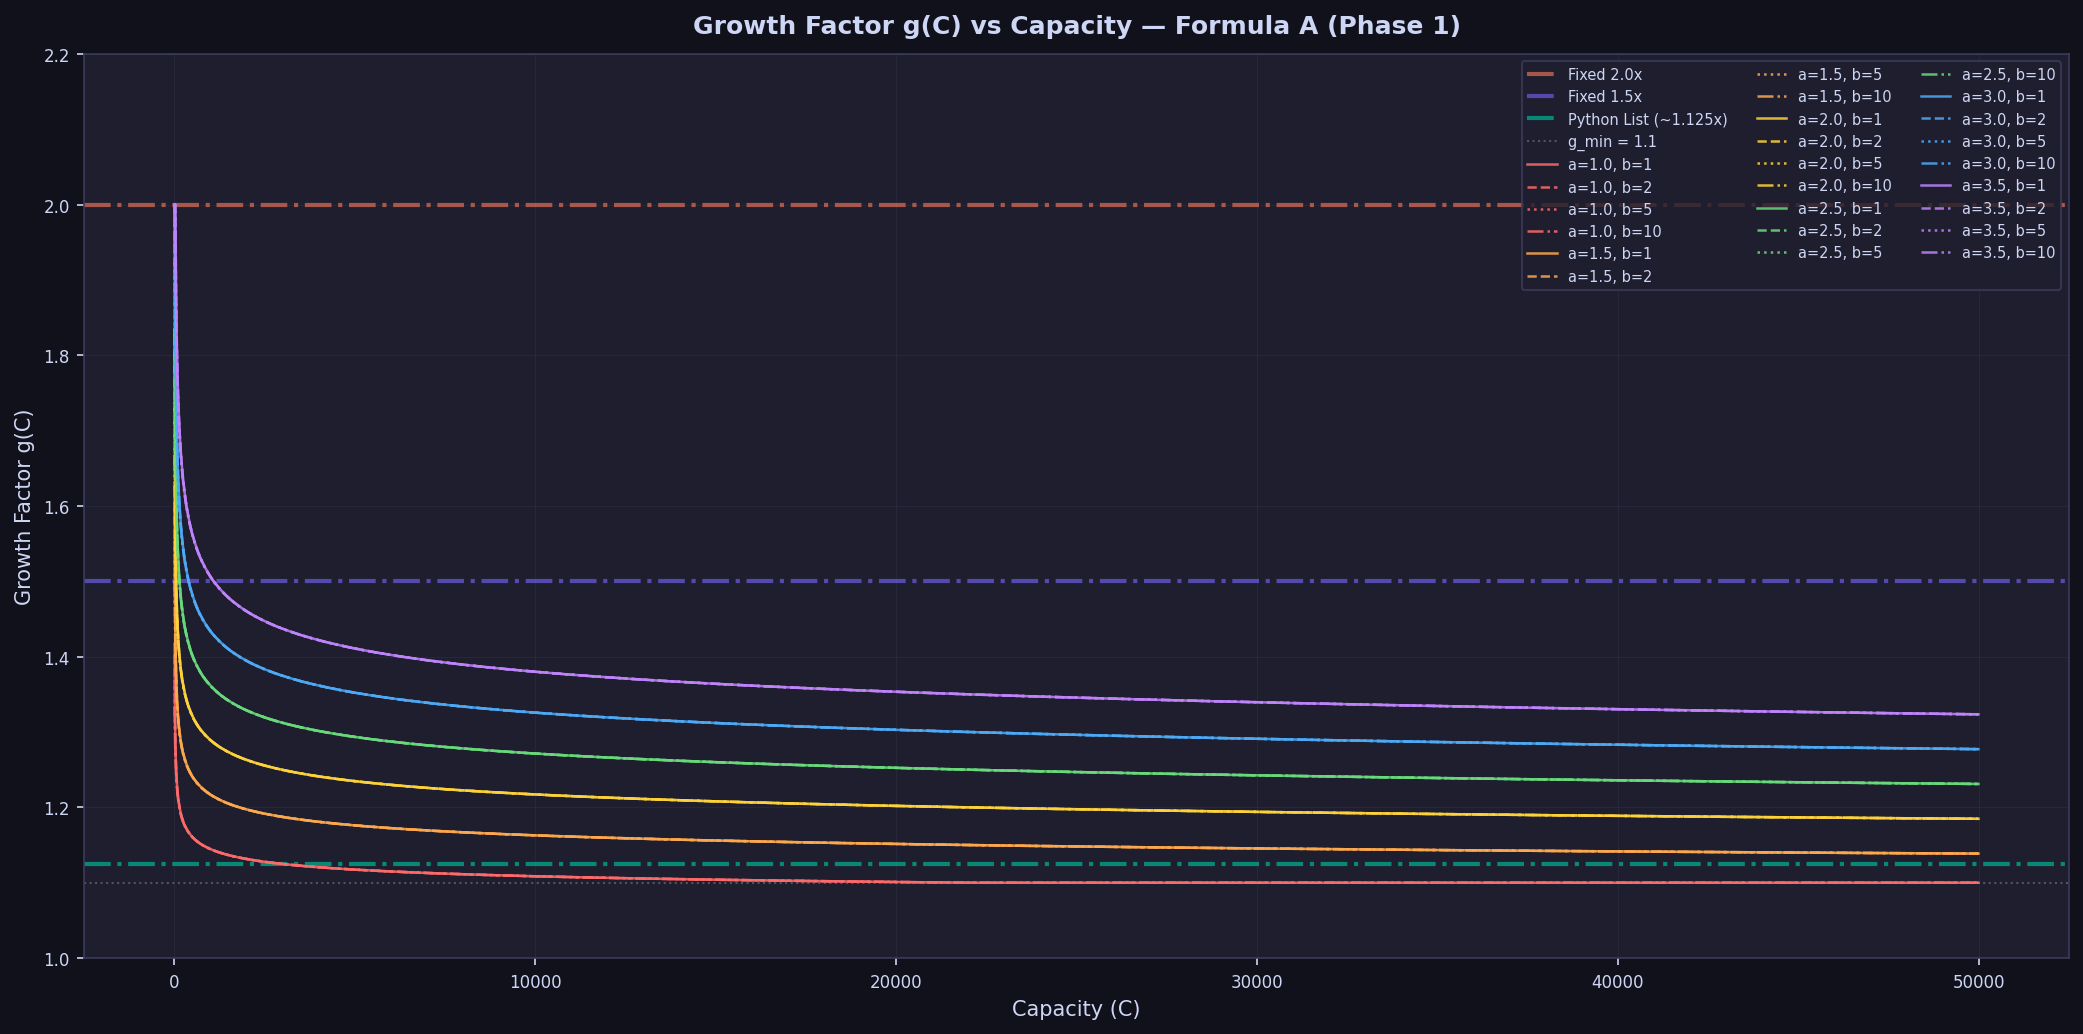
\includegraphics[width=0.7\textwidth]{figures/formula_a_growth_curve.png}
\caption{Growth Factor Decay Curve of Formula A as Capacity Increases}
\label{fig:formula_a_growth}
\end{figure}

As shown in Figure 4.1, the growth factor starts at $2.0$ for small capacities 
and decays toward the $1.1$ clamping limit as the array capacity scales. This 
prevents overallocation at larger scales. During initial resizes (low capacity), 
the absolute memory waste of a $2.0\times$ resize is negligible (e.g., growing 
from 10 to 20 elements wastes only 10 elements). However, at larger capacities, a 
$2.0\times$ resize wastes tens of thousands of elements. Formula A resolves this 
by smoothly shifting to a more conservative growth factor as the capacity increases, 
minimizing final memory waste.

\subsection{Formula B (Harmonic Family)}
Formula B decays the growth factor as a function of the resize count $k$. 
Compared to capacity-dependent decay, decaying based on the resize counter 
ensures a step-wise progression that is independent of the initial allocation size. 
Under Phase 2, when insertion velocity increases, the numerator is boosted:
\begin{equation}
    g(k,v) = 1 + \frac{c_0 + \lambda \ln(1+v)}{k}
\end{equation}
During rapid data ingestion, $\ln(1+v)$ expands, raising the growth factor. 
This allows the array to expand aggressively to skip reallocations during bursts. 
When velocity drops, the growth factor decays harmonically, conserving memory.

\subsection{Formula C and D (Hybrid Frameworks)}
Formula C manually combines the logarithmic and harmonic components, whereas 
Formula D automates hyper-parameter optimization across this space. The 
superiority of Formula D ($J = 0.2589$, $w_A=0.9955, \lambda=3.0944$) is 
visualized in the performance comparisons in Figure 4.6.

\begin{figure}[H]
\centering
\begin{minipage}{0.48\textwidth}
    \centering
    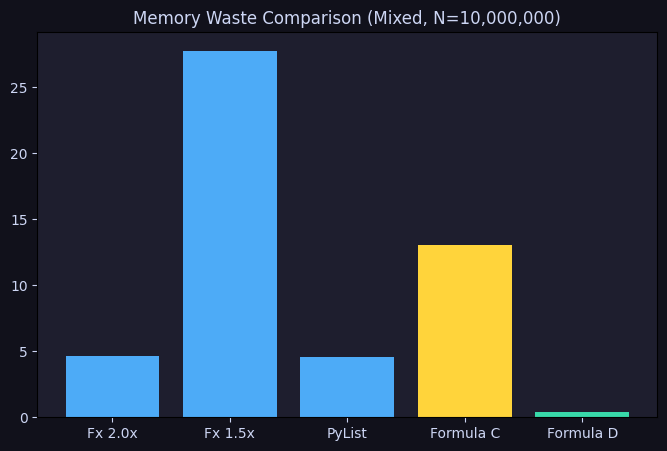
\includegraphics[width=\textwidth]{figures/fd_memory_waste_comparison.png}
    \caption{Memory Waste Comparison}
\end{minipage}\hfill
\begin{minipage}{0.48\textwidth}
    \centering
    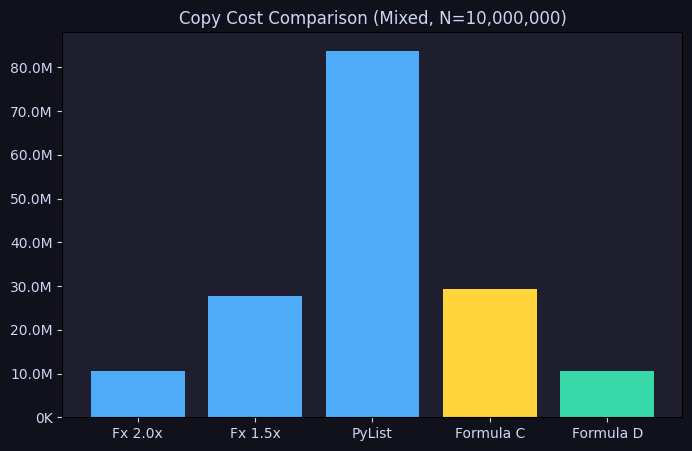
\includegraphics[width=\textwidth]{figures/fd_copy_cost_comparison.png}
    \caption{Copy Cost Comparison}
\end{minipage}
\end{figure}

\begin{figure}[H]
\centering
\begin{minipage}{0.48\textwidth}
    \centering
    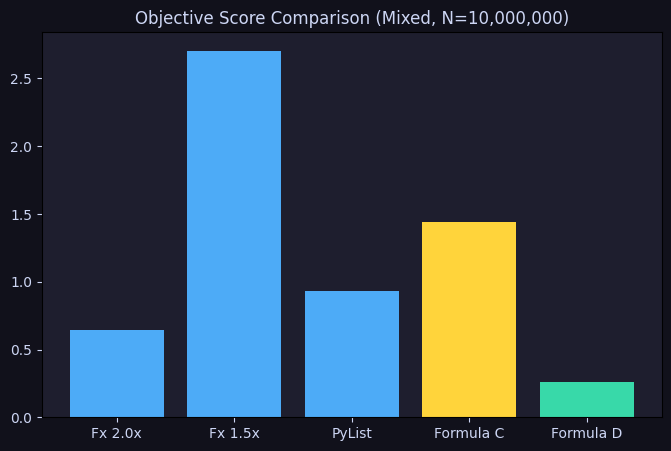
\includegraphics[width=\textwidth]{figures/fd_objective_score_comparison.png}
    \caption{Unified Objective J-Score Comparison}
\end{minipage}\hfill
\begin{minipage}{0.48\textwidth}
    \centering
    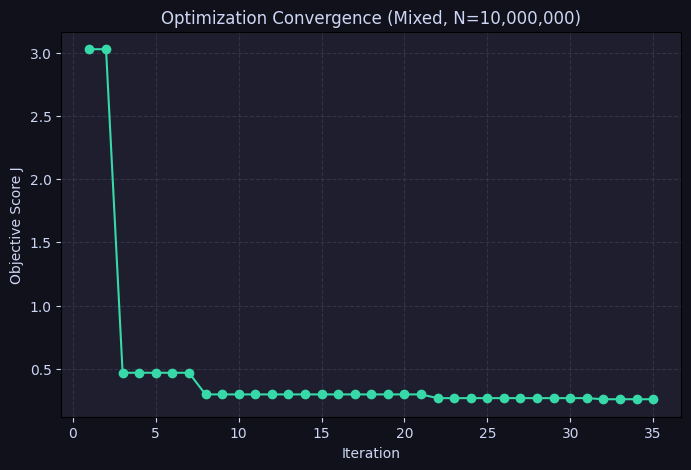
\includegraphics[width=\textwidth]{figures/fd_optimization_convergence.png}
    \caption{GP Bayesian Optimization Convergence}
\end{minipage}
\end{figure}

The charts in Figures 4.2–4.5 show that Formula D achieves a substantial reduction in 
memory waste while maintaining the same copy cost as the Fixed $2.0\times$ 
baseline. This results in the lowest overall $J$-Score. The convergence plot 
(Figure 4.5) indicates that the Gaussian Process model located the minimum 
J-Score within 18 iterations, demonstrating a stable search space.

\section{Parameter Sensitivity Analysis}

\subsection{Sensitivity in Formula A}
To analyze how parameter variations affect the performance of Formula A, we 
swept $\alpha$ and $\beta$ values independently. Figures 4.6 and 4.7 present the 
sensitivity curves.

\begin{figure}[H]
\centering
\begin{minipage}{0.48\textwidth}
    \centering
    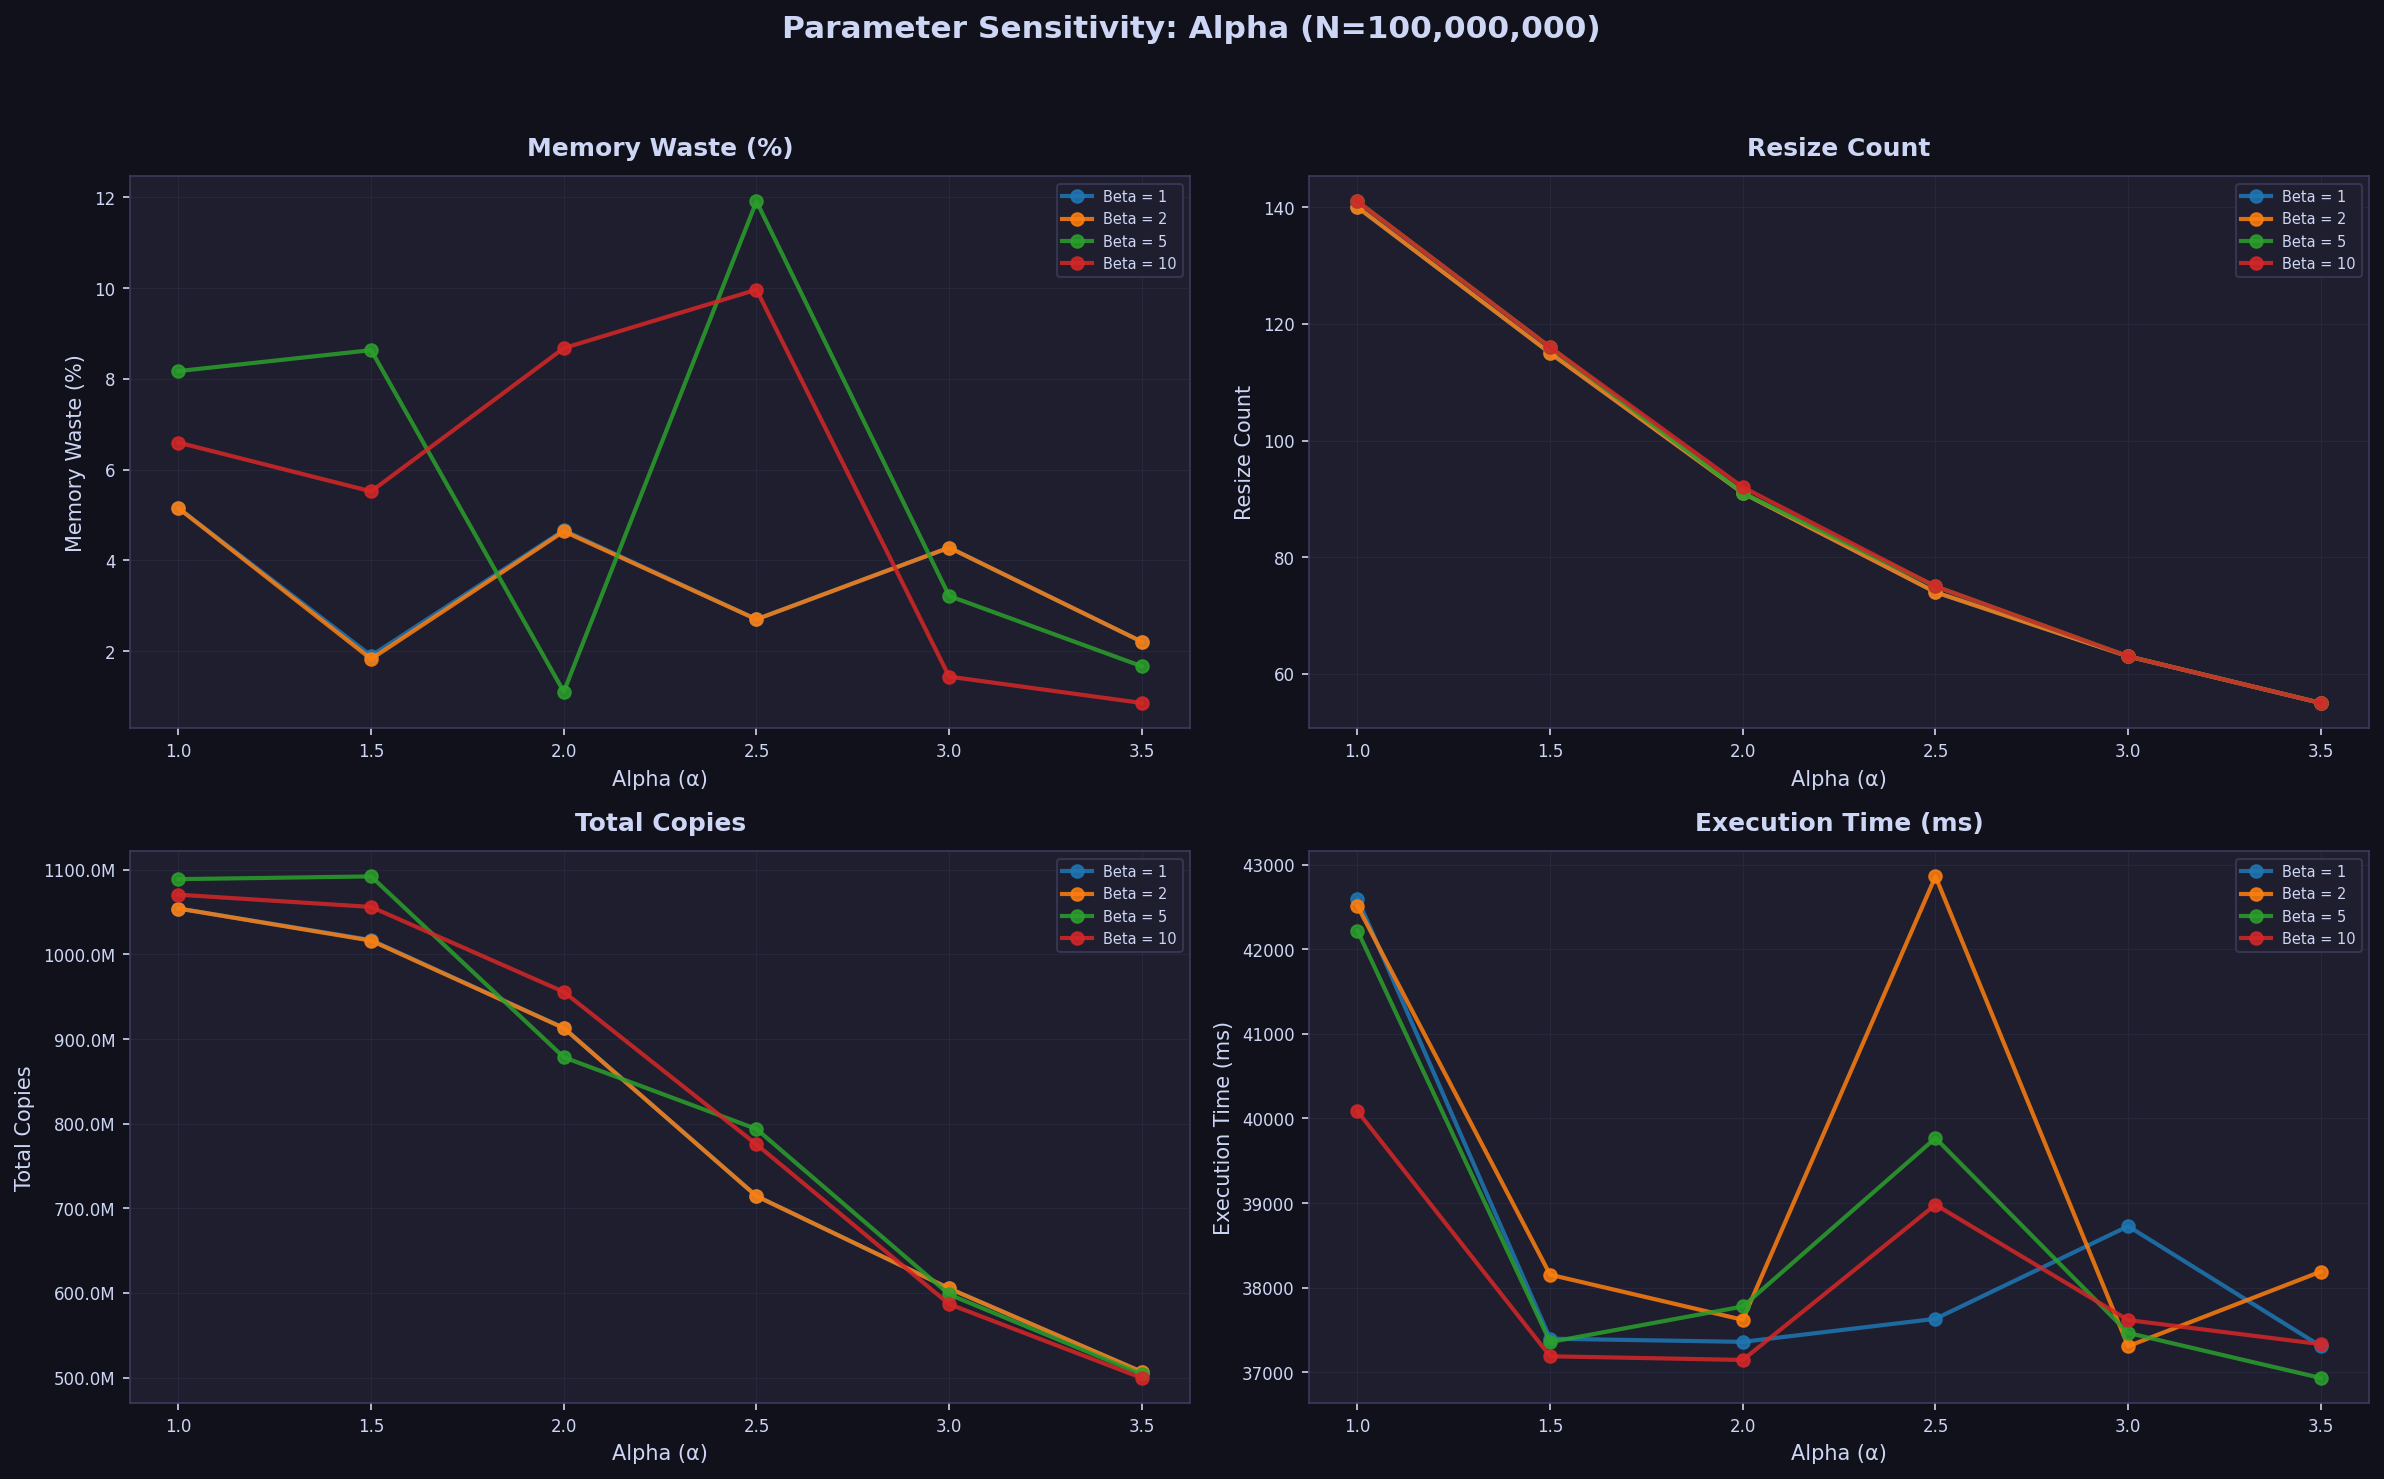
\includegraphics[width=\textwidth]{figures/sensitivity_alpha_100000000.png}
    \caption{Sensitivity of alpha (Formula A)}
\end{minipage}\hfill
\begin{minipage}{0.48\textwidth}
    \centering
    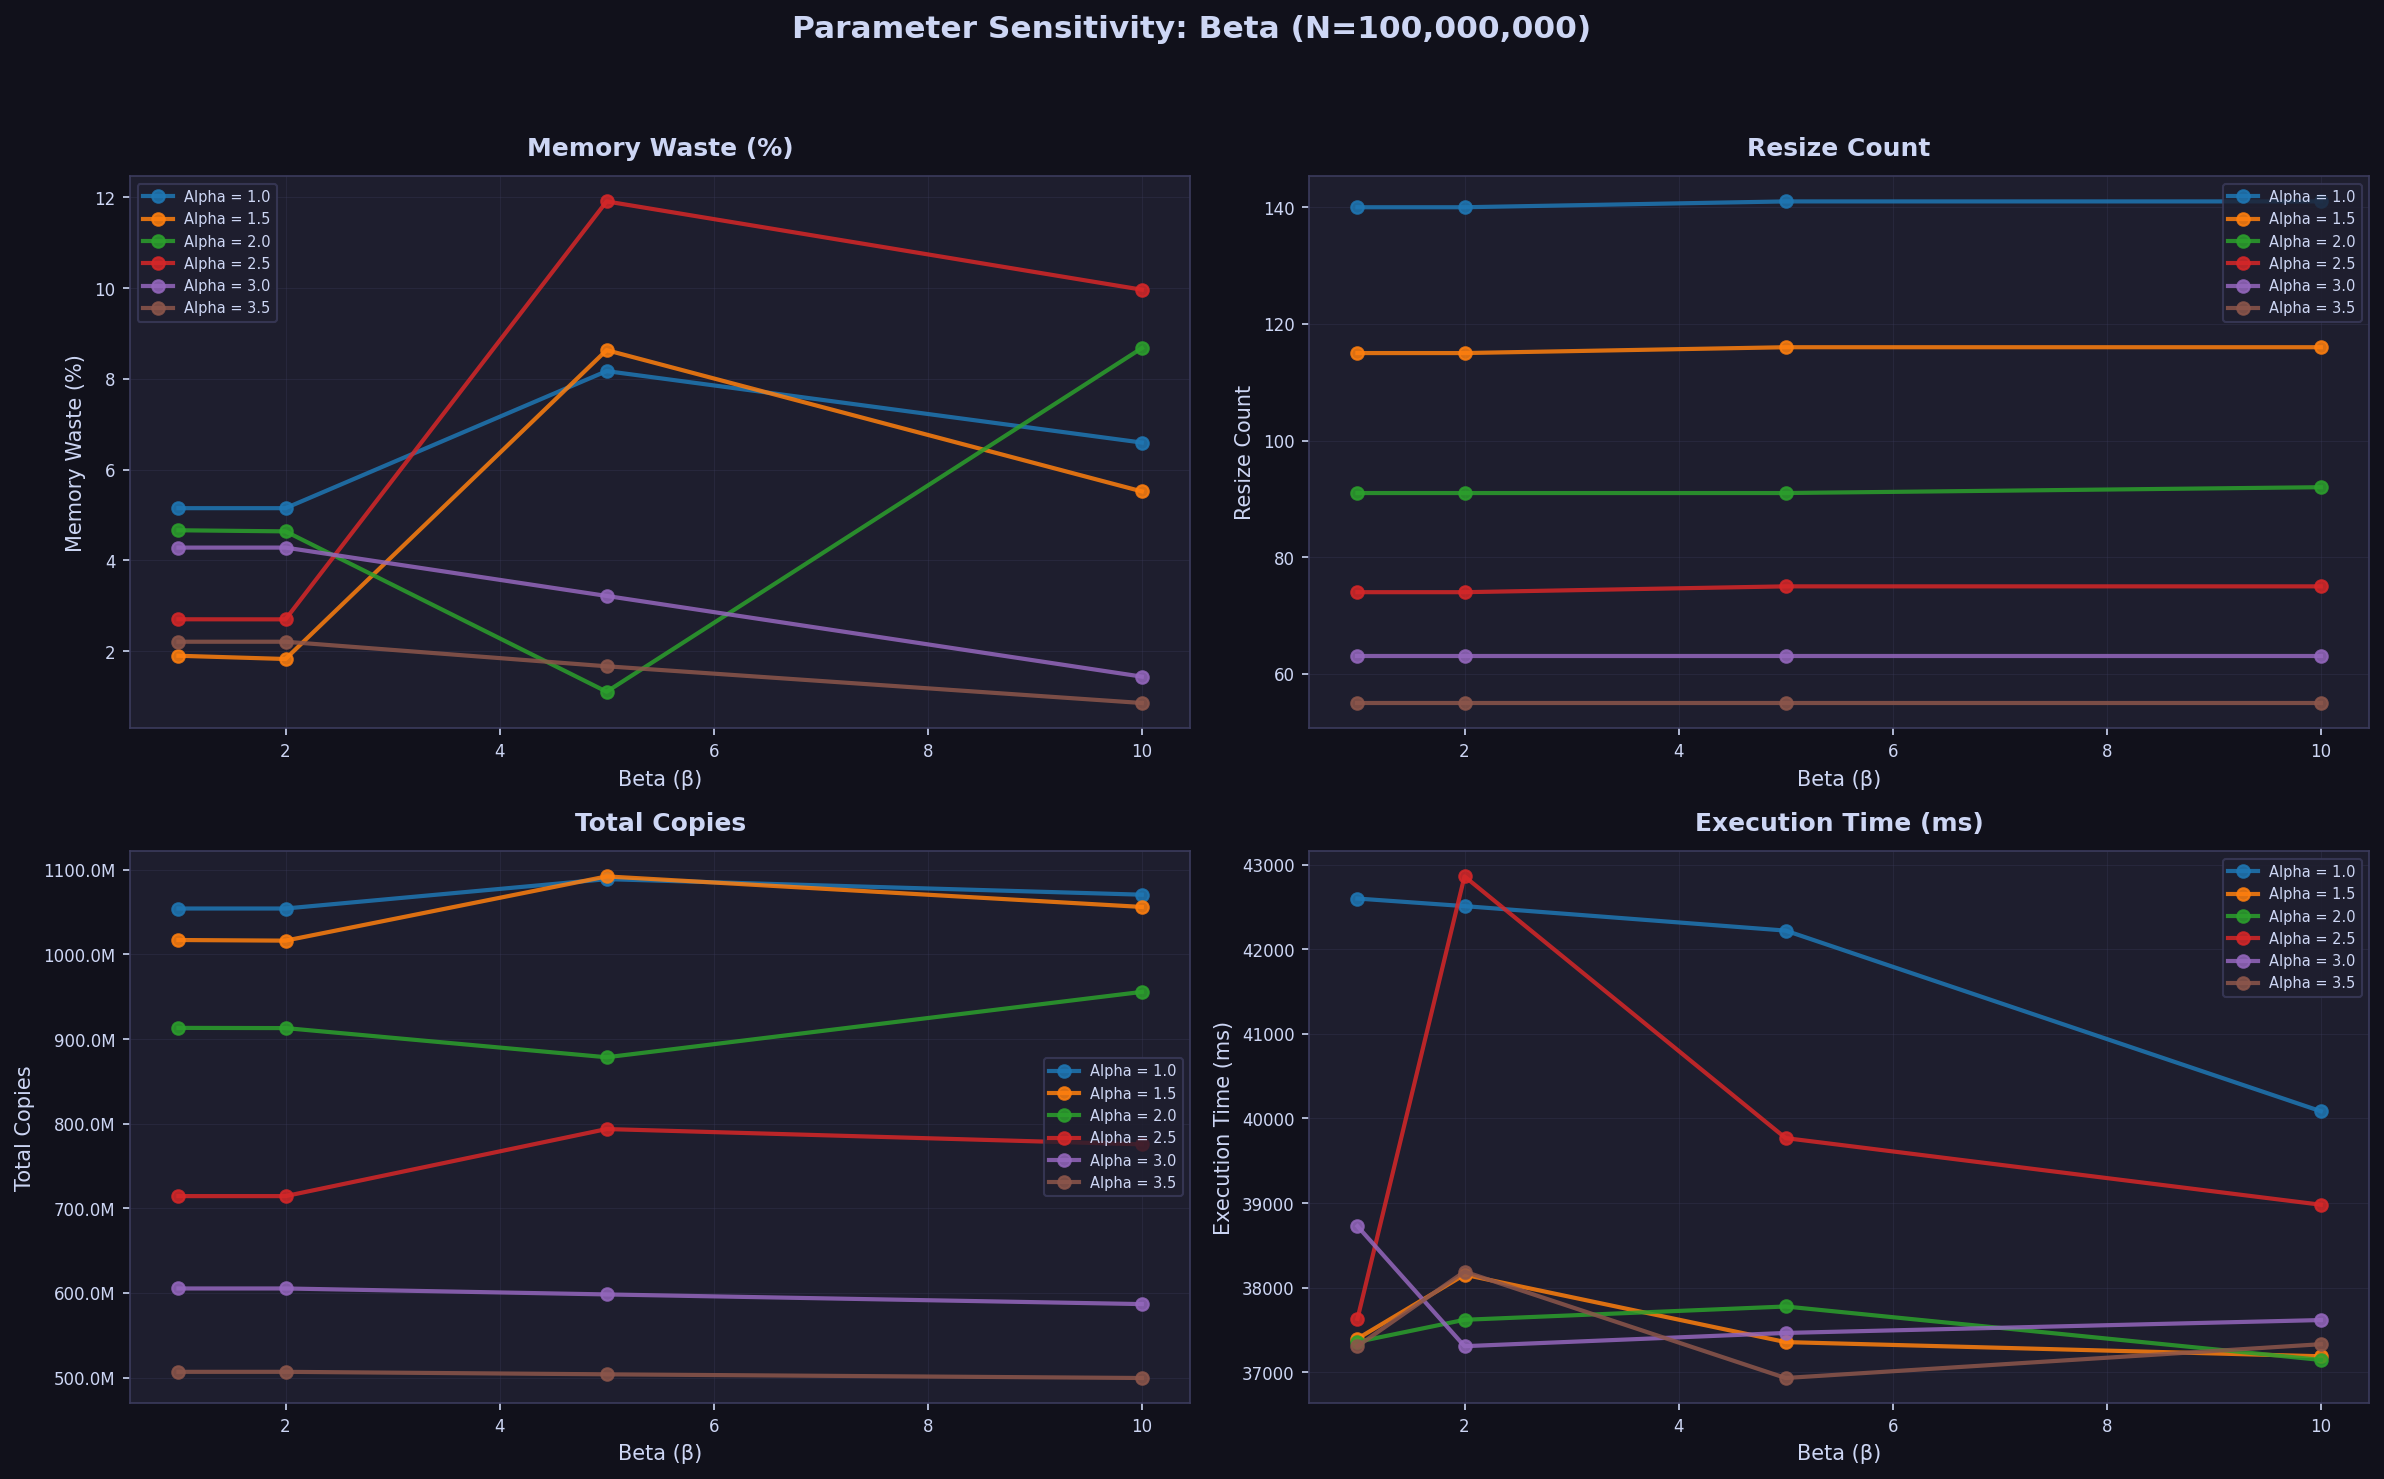
\includegraphics[width=\textwidth]{figures/sensitivity_beta_100000000.png}
    \caption{Sensitivity of beta (Formula A)}
\end{minipage}
\end{figure}

The sensitivity plots reveal that smaller values of $\alpha$ lead to lower 
memory waste but exponentially increase the number of resizes and elements 
copied. The shifting factor $\beta$ acts as a dampener; larger values of $\beta$ 
smooth the decay curve, preventing the growth factor from dropping too rapidly 
during the first few resizes.

\subsection{Sensitivity in Formula B}
For Formula B, we analyzed the sensitivity of the base growth multiplier $c_0$ 
and the velocity weight parameter $\lambda$. Figure 4.8 illustrates the impact 
of these parameters.

\begin{figure}[H]
\centering
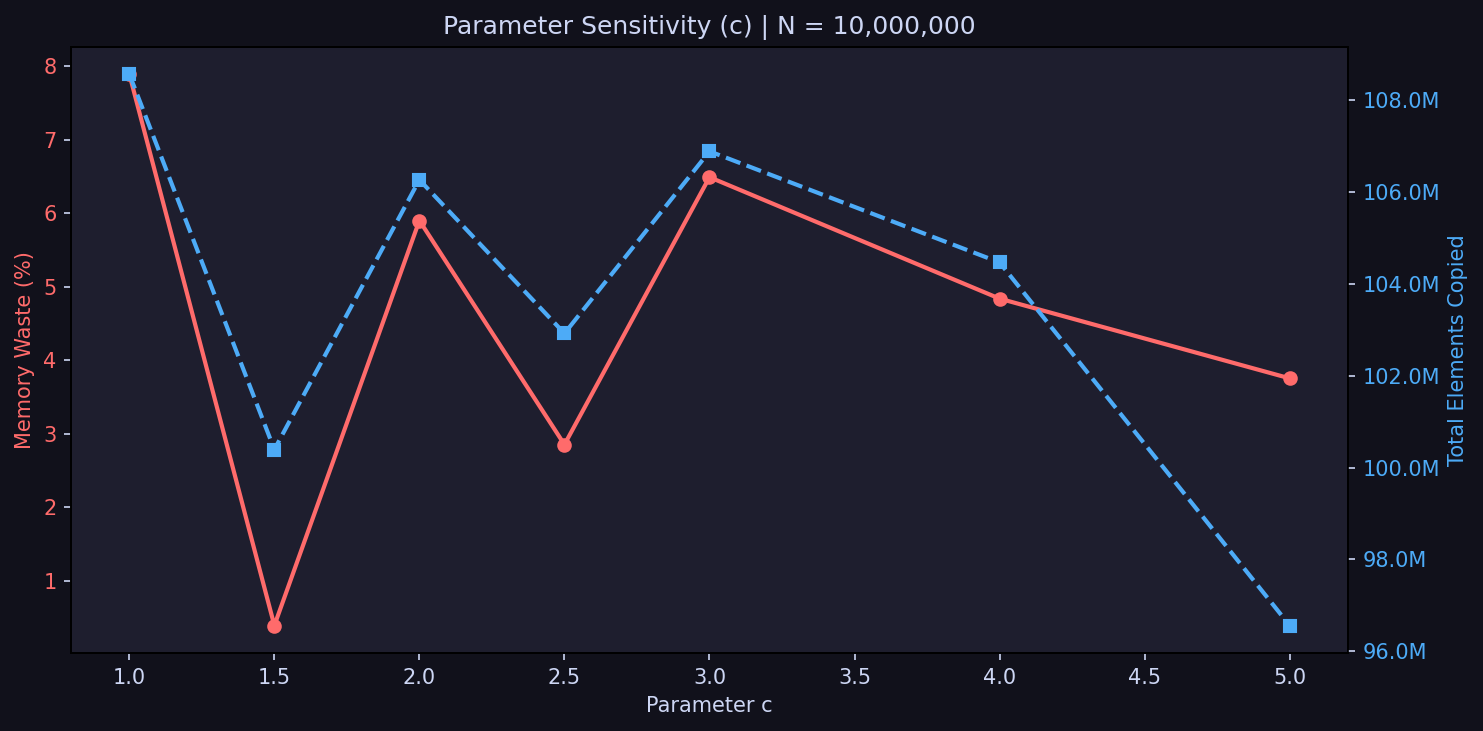
\includegraphics[width=0.7\textwidth]{figures/formula_b_parameter_sensitivity.png}
\caption{Parameter Sensitivity Surface of Formula B}
\label{fig:formula_b_sensitivity}
\end{figure}

\begin{figure}[H]
\centering
\begin{minipage}{0.48\textwidth}
    \centering
    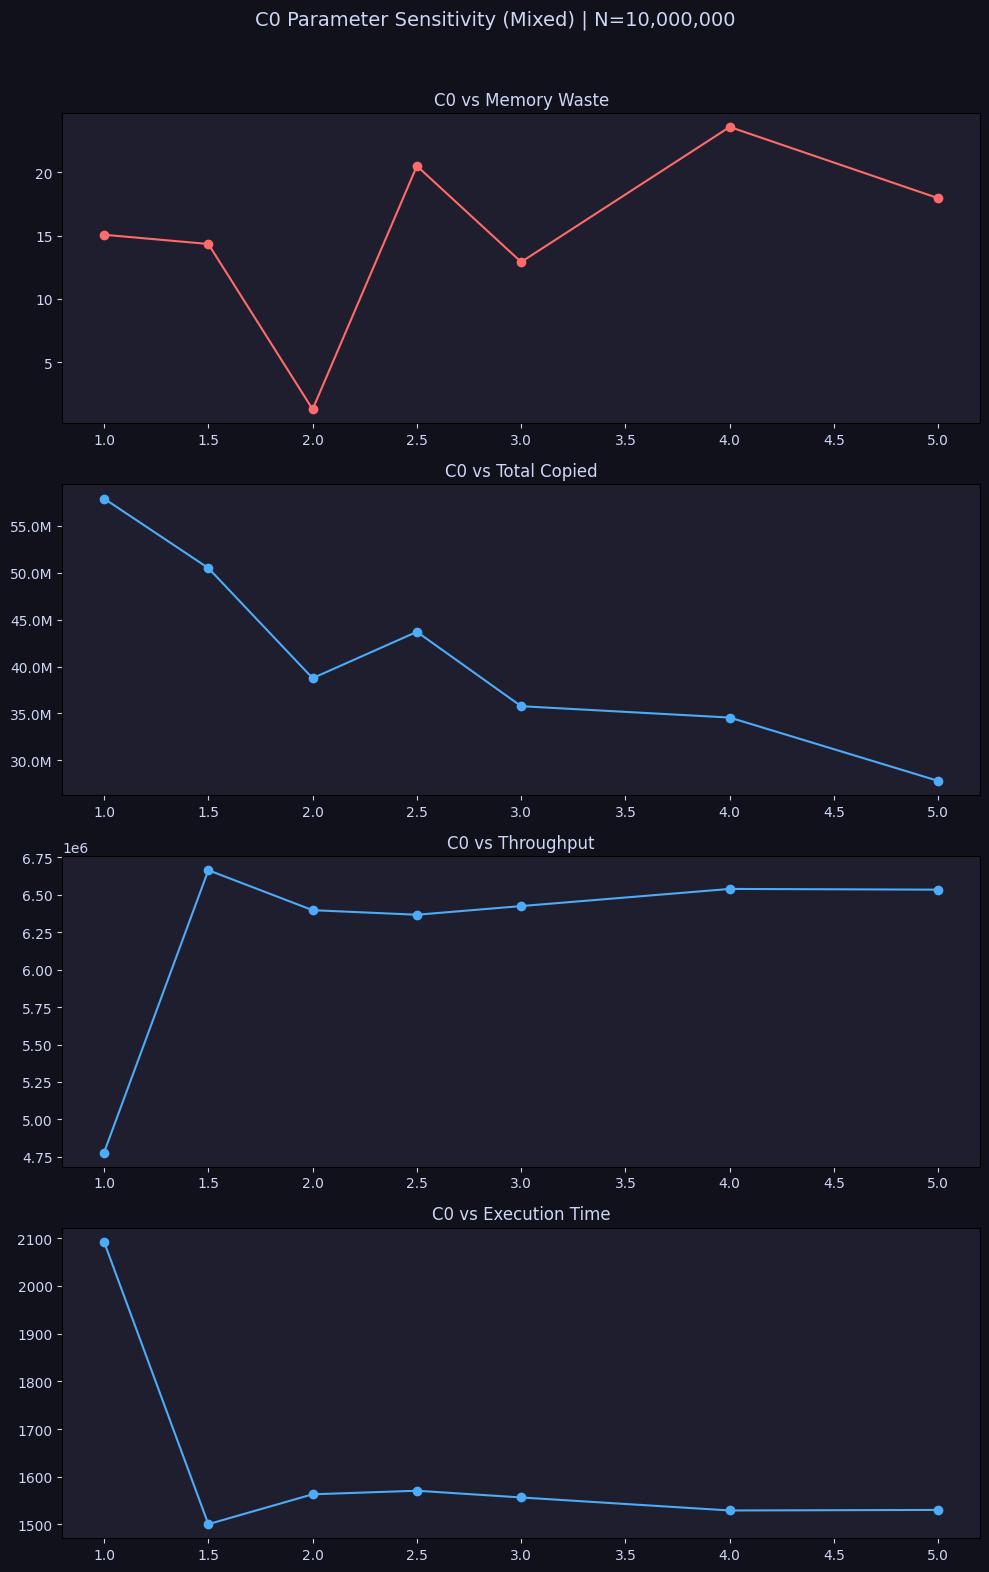
\includegraphics[width=\textwidth]{figures/fb2_c0_sensitivity.png}
    \caption{c0 Sensitivity (Formula B Phase 2)}
\end{minipage}\hfill
\begin{minipage}{0.48\textwidth}
    \centering
    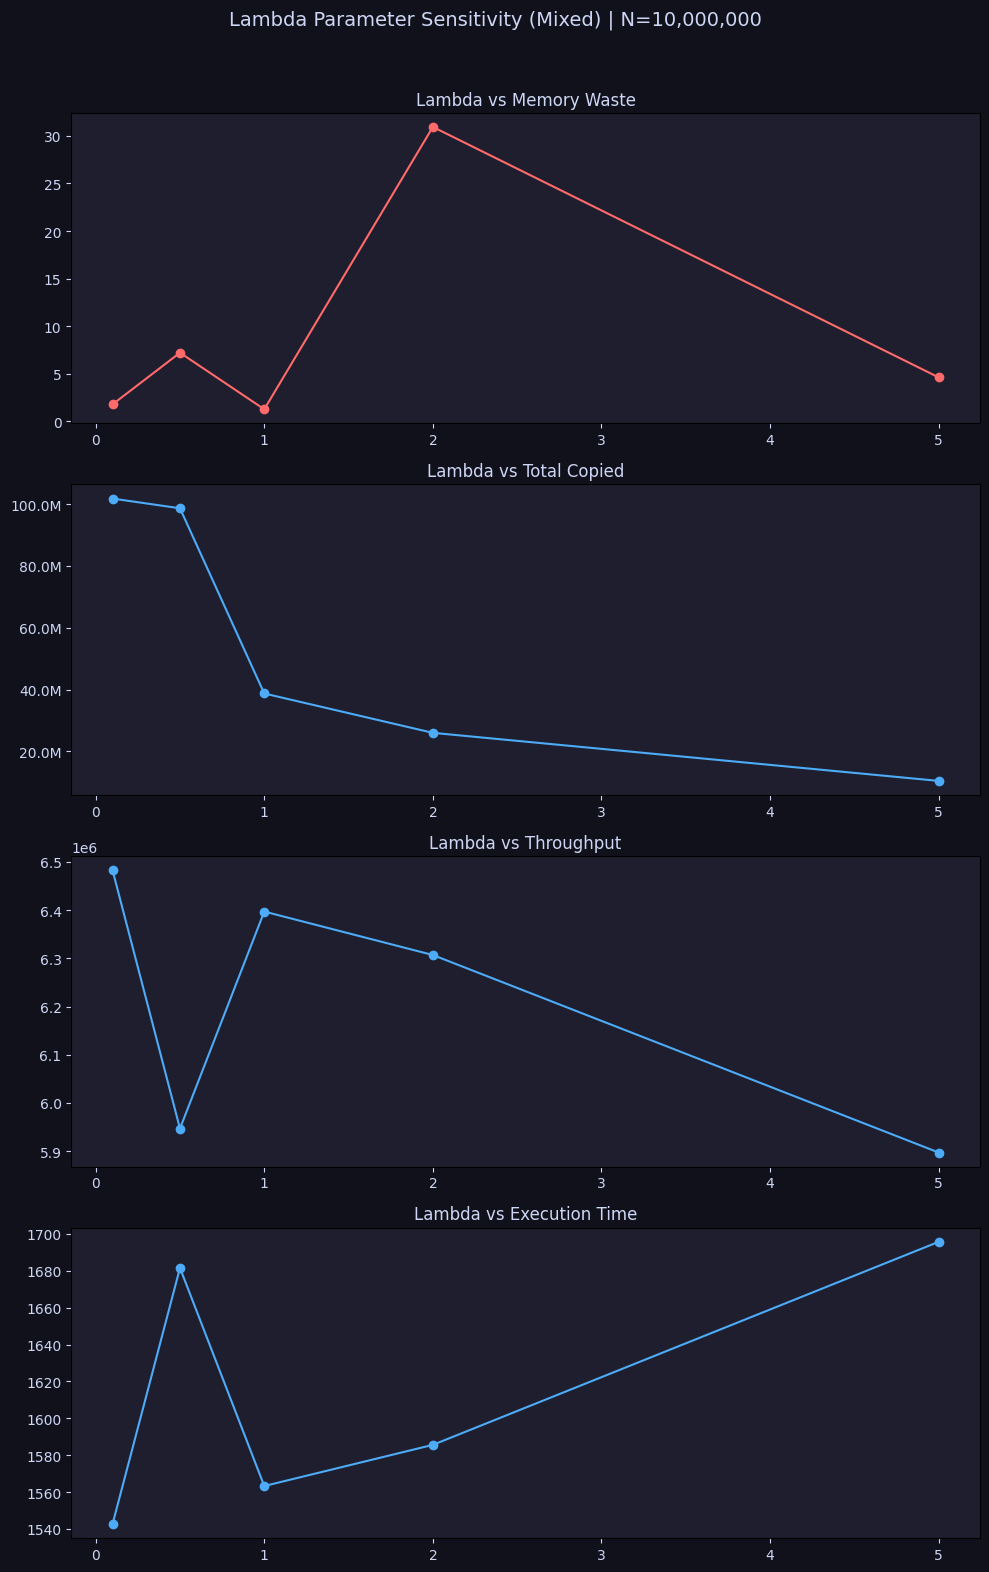
\includegraphics[width=\textwidth]{figures/fb2_lambda_sensitivity.png}
    \caption{Lambda Sensitivity (Formula B Phase 2)}
\end{minipage}
\end{figure}

The sensitivity surface and line plots (Figures 4.9 and 4.10) show that $c_0$ 
dominates the baseline growth rate. A small $c_0$ leads to low waste but high 
copy cost, while a large $c_0$ reduces copies at the expense of higher memory 
waste. The parameter $\lambda$ modulates velocity sensitivity; higher values of 
$\lambda$ allow the algorithm to scale up its expansion factor during burst 
phases, preventing reallocation cascades.

\subsection{Sensitivity in Formula C}
For the manual hybrid model, we evaluated the sensitivity of the weight parameter 
$w_A$ and the velocity parameter $\lambda$. Figures 4.11 and 4.12 show the 
sensitivity trends.

\begin{figure}[H]
\centering
\begin{minipage}{0.48\textwidth}
    \centering
    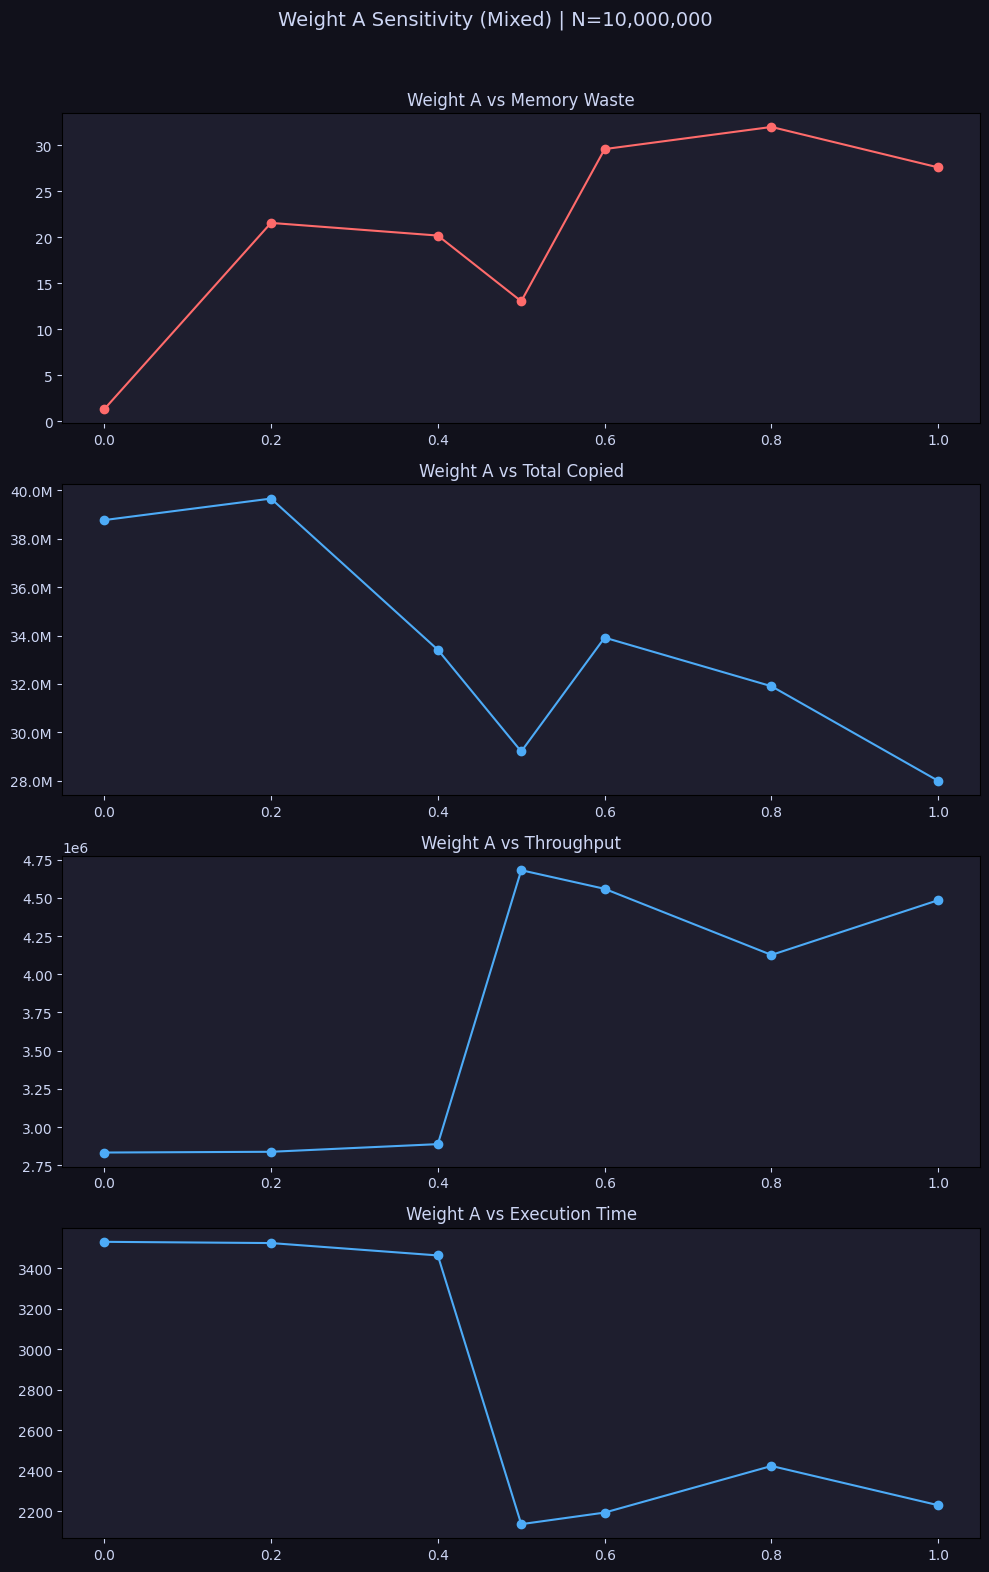
\includegraphics[width=\textwidth]{figures/fc_weighta_sensitivity.png}
    \caption{Weight wA Sensitivity (Formula C)}
\end{minipage}\hfill
\begin{minipage}{0.48\textwidth}
    \centering
    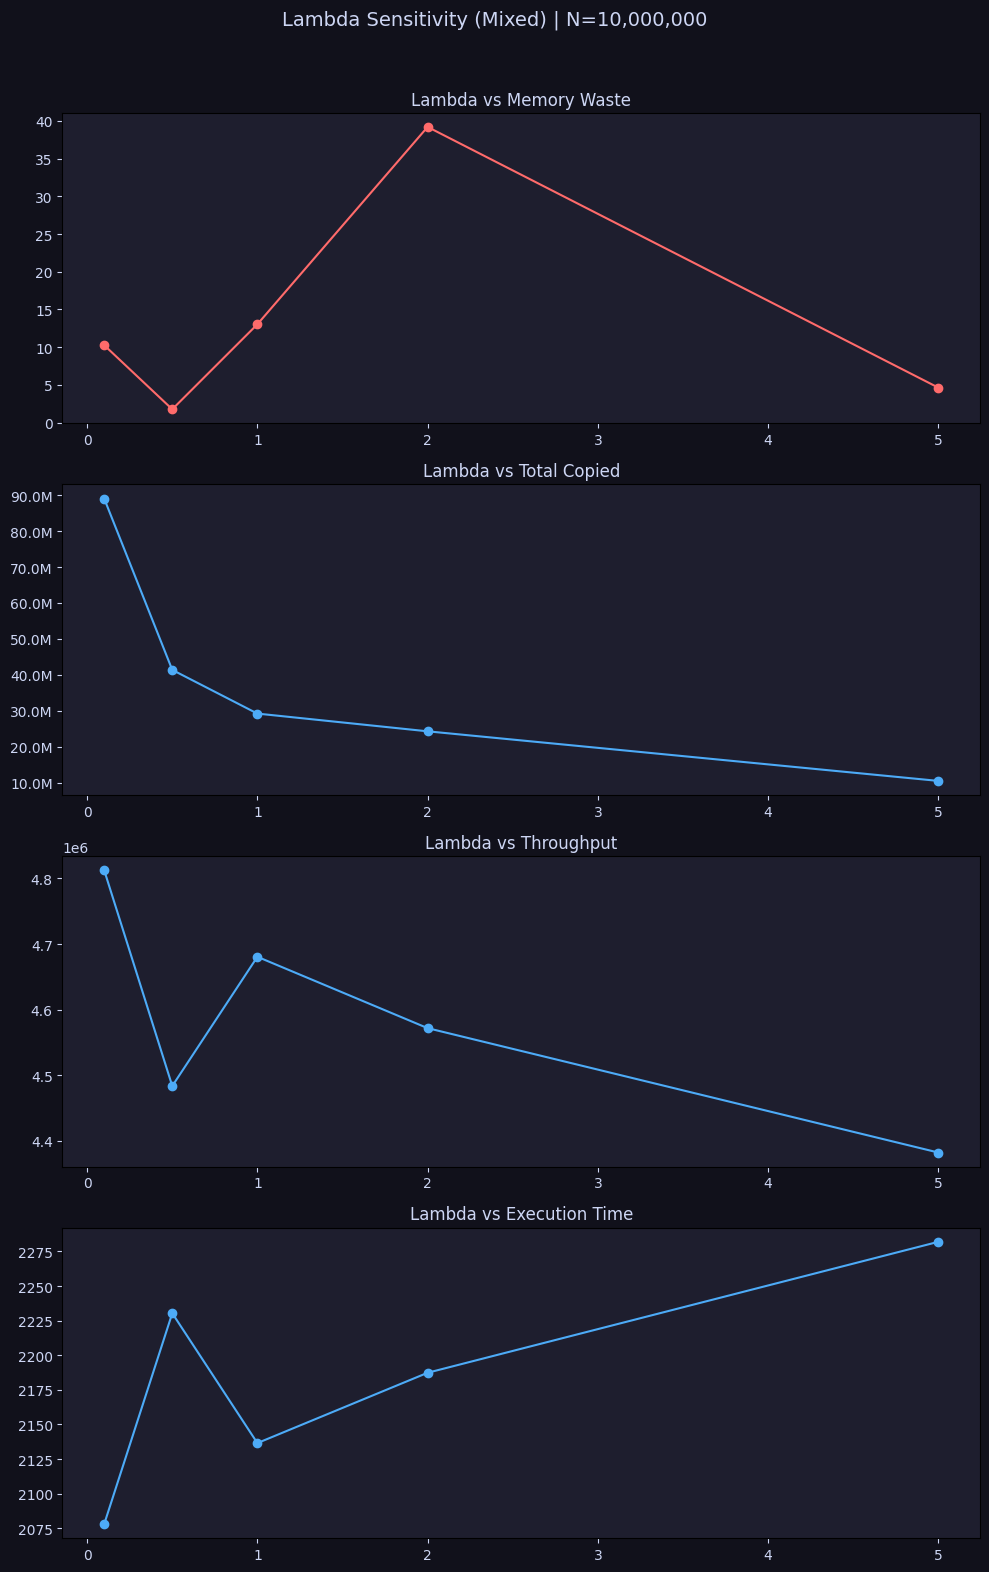
\includegraphics[width=\textwidth]{figures/fc_lambda_sensitivity.png}
    \caption{Lambda Sensitivity (Formula C)}
\end{minipage}
\end{figure}

As shown in Figures 4.11 and 4.12, shifting the weight $w_A$ toward $1.0$ 
increases the influence of the logarithmic component, which leads to a more 
aggressive capacity decay. The parameter $\lambda$ controls the response to 
changes in workload velocity. Optimizing these parameter interactions is key 
to achieving a low $J$-Score, which motivated the development of the automated 
GP-optimization in Formula D.

\section{Summary for the Chapter}
This chapter presented the empirical results and performance evaluations of the 
proposed dynamic array growth algorithms. Section 4.2 presented the Grid Search 
benchmark results, showing that incorporating workload velocity in Phase 2 reduces 
element copying costs while keeping memory waste low. Section 4.3 analyzed the 
Bayesian Optimization results, where the GP-Optimized Hybrid Framework (Formula D) 
achieved the lowest unified objective score ($J=0.2589$). Section 4.4 evaluated 
the logarithmic and harmonic families in detail and performed a sensitivity 
analysis on the key parameters ($\alpha, \beta, c_0, \lambda, w_A$), using 11 
in-depth figures to map the design space. The next chapter summarizes the key 
conclusions and outlines directions for future work.

\chapter{CONCLUSION}

\section{Introduction}
This chapter concludes the research by summarizing the key findings, drawing 
empirical conclusions, outlining the limitations of the current work, and 
identifying potential directions for future research. The core focus of this 
dissertation was to address the inefficiencies of standard dynamic array 
resizing policies, which rely on rigid, workload-independent growth factors 
(e.g., $1.5\times$ or $2.0\times$). By introducing runtime feedback loops that 
incorporate resize history ($k$) and real-time insertion velocity ($v$), this 
study successfully developed and optimized an adaptive resizing framework that 
balances memory efficiency and computational speed.

\section{Summary of Findings}
The empirical results compiled across $10^7$ element benchmarks (detailed in 
Chapter 4) demonstrate the high efficiency of the proposed workload-aware 
resizing models. The key findings of this research are summarized below:
\begin{itemize}
    \item \textbf{Optimal Overall Model:} The GP-Optimized Hybrid Framework 
    (Formula D) achieved the lowest overall cost score, $J = 0.2589$. With optimized 
    parameters ($w_A = 0.9955$, $\lambda = 3.0944$), Formula D restricted 
    memory waste to a mere \textbf{0.42\%} while requiring only \textbf{20 resizes} 
    and \textbf{10.49M elements copied}. This matched the optimal copy speed 
    of the C++ STL doubling policy ($2.0\times$) while reducing final memory 
    waste by \textbf{90.9\%} (from 4.63\% down to 0.42\%).
    \item \textbf{Comparison with Static Standards:} Compared to other industry 
    standards, the proposed Formula D demonstrated substantial improvements:
    \begin{itemize}
        \item It reduced memory waste by \textbf{98.5\%} compared to Java's 
        $1.5\times$ policy (27.77\% waste) and cut element copying overhead by 
        \textbf{62.1\%} (from 27.69M copies down to 10.49M).
        \item It reduced cumulative element copies by \textbf{87.5\%} compared 
        to CPython's list policy (83.84M copies down to 10.49M) while maintaining 
        comparable memory utilization.
    \end{itemize}
    \item \textbf{Absolute Memory Waste Leader:} The Bayesian-tuned Formula A 
    Phase 1 (Logarithmic) achieved the lowest absolute memory waste of \textbf{0.05\%} 
    at the end of insertion, demonstrating the theoretical limit of capacity-based 
    decay, albeit at the cost of 32.31M element copies.
    \item \textbf{Workload Adaptability:} The feedback-enabled models successfully 
    adapted to diverse data ingestion profiles. By incorporating velocity $v$, the 
    array expanded aggressively during high-speed burst phases to skip costly 
    reallocations, and grew conservatively during slow, sparse insertion phases 
    to prevent over-allocation.
\end{itemize}

\section{Conclusion Drawn by Results}
Based on the empirical evidence, several conclusions can be drawn:
\begin{enumerate}
    \item \textbf{Effectiveness of the Proposed Strategy:} The research successfully 
    proved that incorporating runtime feedback of resize history 
    and insertion velocity allows dynamic arrays to achieve a superior trade-off 
    between spatial and temporal efficiency compared to static, fixed growth 
    factors.
    \item \textbf{Harmonic Decay is Highly Effective:} Decaying the growth 
    factor harmonically based on the resize counter ($k$) is an extremely effective 
    mechanism for contiguous arrays. It naturally limits the absolute volume of 
    wasted space as the array grows massive, preventing the geometric waste 
    accumulation seen in standard doubling policies.
    \item \textbf{Throughput Preservation:} The computational overhead of evaluating 
    logarithmic and harmonic math operations during resize events is negligible 
    when compared to the massive time savings achieved by avoiding memory allocation 
    calls and element copying loops. Thus, adaptive resizing improves overall 
    efficiency without sacrificing throughput.
\end{enumerate}

\section{Limitations}
While the proposed algorithm demonstrated high efficiency, several limitations 
were identified during this study:
\begin{itemize}
    \item \textbf{Timestamp Measurement Overhead:} Querying the high-resolution 
    system clock (\texttt{time.perf\_counter()}) to compute insertion velocity 
    introduces a small but non-zero CPU overhead during each resize cycle. In 
    extremely high-performance systems with tiny arrays, this system call latency 
    can slightly degrade throughput.
    \item \textbf{Simulation Boundaries:} The evaluation was conducted inside 
    a custom Python-based simulation environment. Although the simulator accurately 
    models logical capacity, size, and element copying overheads, it operates 
    within CPython's managed memory heap. The actual physical memory layout and 
    virtual memory fragmentation are thus dependent on CPython's garbage collector, 
    introducing minor measurement noise.
    \item \textbf{Static Clamping Bounds:} The lower and upper clamping bounds 
    ($g_{\min} = 1.1$, $g_{\max} = 2.0$) were set statically. In systems with 
    highly unusual memory pages, these bounds may need to be adjusted dynamically.
\end{itemize}

\section{Future Works}
To address the limitations and expand the applicability of this research, 
the following areas are proposed for future study:
\begin{itemize}
    \item \textbf{Native C++ STL Integration:} Porting the adaptive growth 
    engine directly into a custom C++ STL allocator or modifying the 
    \texttt{std::vector} implementation. Testing in a compiled language will 
    eliminate runtime interpreter noise and allow measuring raw, bare-metal CPU 
    execution cycles.
    \item \textbf{Deployment in Embedded Systems (IoT):} Evaluating the 
    algorithm on resource-constrained microcontrollers (e.g., ESP32, ARM Cortex-M) 
    where memory is highly restricted (measured in kilobytes) and memory 
    fragmentation can lead to system crashes.
    \item \textbf{Predictive Machine Learning Models:} Replacing the simple 
    historical velocity averages with lightweight online regression or reinforcement 
    learning models that can predict upcoming data bursts, allowing the array to 
    pre-allocate memory preemptively.
    \item \textbf{Multi-Threaded Vector Optimizations:} Extending the velocity 
    computations to support thread-safe, lock-free concurrent vector structures, 
    adjusting the growth factor based on collective thread insertion speeds.
\end{itemize}

\section{Summary for the Chapter}
This chapter concluded the research by summarizing the findings and drawing 
conclusions on workload-aware dynamic array resizing. Section 5.2 summarized the 
empirical findings, highlighting that the GP-Optimized Hybrid Framework 
(Formula D) achieved a Pareto-optimal J-Score of 0.2589, cutting memory waste 
by 90.9\% compared to C++ doubling while matching its copy speed. Section 5.3 
validated the core design strategy, confirming that harmonic resize decay 
coupled with velocity scaling balances space and time effectively. Section 5.4 
discussed current limitations, including clock measurement overhead and simulation 
boundaries. Finally, Section 5.5 outlined future directions, including C++ STL 
vector integration, embedded IoT deployments, and predictive models, providing 
a clear roadmap for subsequent research.


\newpage
\addcontentsline{toc}{chapter}{REFERENCES}
\begin{thebibliography}{26}

\bibitem{java_data_structures}
D.~E. Costa, A.~Andrzejak, J.~Seboek, and D.~Lo, ``Empirical Study of Usage and Performance of Java Collections,'' in \emph{Proc. 8th ACM/SPEC Int. Conf. Performance Engineering (ICPE)}, 2017, pp. 389--400.

\bibitem{time_space_complexity}
R.~E. Tarjan and U.~Zwick, ``Optimal Resizable Arrays,'' in \emph{Proc. 5th Symp. Simplicity in Algorithms (SOSA)}, 2023, pp. 1--10.

\bibitem{optimal_resizable}
A.~Brodnik, S.~Carlsson, E.~D. Demaine, J.~I. Munro, and R.~Sedgewick, ``Resizable Arrays in Optimal Time and Space,'' in \emph{Proc. 6th Int. Workshop Algorithms and Data Structures (WADS)}, 1999, pp. 37--48.

\bibitem{resizable_optimal_time_space}
P.~Bille, A.~R. Christiansen, M.~B. Ettienne, and I.~L. G{\o}rtz, ``Fast Dynamic Arrays,'' in \emph{Proc. 25th Annual European Symposium on Algorithms (ESA)}, 2017, pp. 16:1--16:14.

\bibitem{allocating_storage}
A.~L. Rosenberg, ``Allocating Storage for Extendible Arrays,'' \emph{Journal of the ACM}, vol. 21, no. 4, pp. 652--670, 1974.

\bibitem{managing_storage}
A.~L. Rosenberg, ``Managing Storage for Extendible Arrays,'' \emph{SIAM Journal on Computing}, vol. 4, no. 3, pp. 287--306, 1975.

\bibitem{fast_array}
J.~Katajainen, ``Worst-case-efficient Dynamic Arrays in Practice,'' in \emph{Proc. 15th Int. Symposium on Experimental Algorithms (SEA)}, 2016, pp. 202--217.

\bibitem{adaptive_packed}
M.~A. Bender, R.~Cole, E.~D. Demaine, and M.~Farach-Colton, ``Adaptive Packed Memory Array,'' \emph{ACM Transactions on Database Systems}, vol. 30, no. 4, pp. 110--128, 2005.

\bibitem{trends_adaptive}
H.~Singh and R.~M. Jha, ``Trends in Adaptive Array Processing,'' \emph{International Journal of Antennas and Propagation}, vol. 2012, pp. 1--11, 2012.

\bibitem{black_white_array}
Z.~G. Mou, ``Black-White Array: A New Data Structure for Dynamic Data Sets,'' \emph{arXiv preprint arXiv:cs/0409051}, pp. 1--15, 2004.

\bibitem{z_rays}
J.~B. Sartor, S.~M. Blackburn, D.~Frampton, M.~Hirzel, and K.~S. McKinley, ``Z-rays: Divide Arrays and Conquer Speed and Flexibility,'' in \emph{Proc. 31st ACM SIGPLAN Conf. Programming Language Design and Implementation (PLDI)}, 2010, pp. 406--417.

\bibitem{logarithmic_arrays}
R.~R. Hoogerwoord, ``A Logarithmic Implementation of Flexible Arrays,'' in \emph{Proc. 2nd International Conference on Mathematics of Program Construction (MPC)}, 1992, pp. 191--207.

\bibitem{lock_free_vector}
D.~Dechev, P.~Pirkelbauer, and B.~Stroustrup, ``Lock-Free Dynamically Resizable Arrays,'' in \emph{Proc. 10th International Conference on Principles of Distributed Systems (OPODIS)}, 2006, pp. 142--156.

\bibitem{persistent_arrays}
P.~F. Dietz, ``Fully Persistent Arrays,'' in \emph{Proc. 1st Workshop on Algorithms and Data Structures (WADS)}, 1989, pp. 67--74.

\bibitem{query_processing}
P.~Baumann, A.~Dehmel, P.~Furtado, R.~Ritsch, and N.~Widmann, ``The Multidimensional Database System RasDaMan,'' in \emph{Proc. 1998 ACM SIGMOD International Conference on Management of Data}, 1998, pp. 575--577.

\bibitem{cormen_algorithms}
T.~H. Cormen, C.~E. Leiserson, R.~L. Rivest, and C.~Stein, \emph{Introduction to Algorithms}, 4th~ed. Cambridge, MA, USA: MIT Press, 2022.

\bibitem{python_list_impl}
Python Software Foundation, ``CPython List Object Implementation,'' CPython Source Code, GitHub Repository, \texttt{listobject.c}, 2023.

\bibitem{practical_bayesian_opt}
J.~Snoek, H.~Larochelle, and R.~P. Adams, ``Practical Bayesian Optimization of Machine Learning Algorithms,'' in \emph{Proc. 25th International Conference on Neural Information Processing Systems (NIPS)}, 2012, pp. 2951--2959.

\bibitem{bayesian_opt_review}
B.~Shahriari, K.~Swersky, Z.~Wang, R.~P. Adams, and N.~de Freitas, ``Taking the Human Out of the Loop: A Review of Bayesian Optimization,'' \emph{Proceedings of the IEEE}, vol. 104, no. 1, pp. 148--175, 2016.

\bibitem{dynamic_storage_allocation}
P.~R. Wilson, M.~S. Johnstone, M.~Neely, and D.~Boles, ``Dynamic Storage Allocation: A Survey and Critical Review,'' in \emph{Proc. 1st International Workshop on Memory Management (IWMM)}, 1995, pp. 1--116.

\bibitem{reconsidering_custom_allocation}
E.~D. Berger, B.~G. Zorn, and K.~S. McKinley, ``Reconsidering Custom Memory Allocation,'' in \emph{Proc. 17th ACM SIGPLAN Conference on Object-Oriented Programming, Systems, Languages, and Applications (OOPSLA)}, 2002, pp. 1--12.

\bibitem{frigo_cache_oblivious}
M.~Frigo, C.~E. Leiserson, H.~Prokop, and S.~Ramachandran, ``Cache-Oblivious Algorithms,'' in \emph{Proc. 40th Annual Symposium on Foundations of Computer Science (FOCS)}, 1999, pp. 285--297.

\bibitem{python_malloc_impl}
Python Software Foundation, ``CPython Object Allocator Implementation,'' CPython Source Code, GitHub Repository, \texttt{obmalloc.c}, 2023.

\bibitem{scikit_optimize}
T.~Head, M.~Kumar, H.~Nahrstaedt, G.~Louppe, and I.~Shcherbatyi, ``scikit-optimize: Sequential model-based optimization in Python,'' Zenodo, \texttt{https://github.com/scikit-optimize/scikit-optimize}, 2018.

\bibitem{jones_ego}
D.~R. Jones, M.~Schonlau, and W.~J. Welch, ``Efficient Global Optimization of Expensive Black-Box Functions,'' \emph{Journal of Global Optimization}, vol. 13, no. 4, pp. 455--492, 1998.

\bibitem{hoard_allocator}
E.~D. Berger, K.~S. McKinley, R.~D. Blumofe, and P.~R. Wilson, ``Hoard: A Scalable Memory Allocator for Multithreaded Applications,'' in \emph{Proc. 9th International Conference on Architectural Support for Programming Languages and Operating Systems (ASPLOS)}, 2000, pp. 117--128.

\end{thebibliography}


\chapter*{APPENDIX A: PYTHON SIMULATOR SOURCE CODE}
\addcontentsline{toc}{chapter}{APPENDIX A: PYTHON SIMULATOR SOURCE CODE}

To ensure reproducibility and transparency, the complete Python source code for 
the benchmarking dynamic array simulator and the Gaussian Process Bayesian 
Optimization loop is presented below. This code contains the implementation of 
the seven data ingestion profiles, the virtual memory resize simulation, and 
the objective $J$-Score evaluation framework.

\lstinputlisting[language=Python, caption={Core Simulation and Optimization Script (formula\_d.py)}]{appendices/formula_d.py}


\end{document}
